\documentclass[12pt]{article}
\usepackage[utf8]{inputenc}
\usepackage[a4paper,margin=1in]{geometry}
\usepackage{hyperref}
\usepackage{graphicx}
\usepackage{booktabs}
\usepackage{amsmath}
\usepackage{caption}
\usepackage{float}
\usepackage[superscript]{cite}

\title{Project Report}
\author{%
  \textbf{Prepared by:} Warul Kumar Sinha (2023201045)\\
  \textbf{Under the advisory of:} Dr.\ Kshitij Gajjar
}
\date{}

\begin{document}

\maketitle
\thispagestyle{empty}

\noindent A variety of algorithms exist to solve the same problem, but nuances often affect practical applicability. This project aims to analyse, benchmark, compare, and document algorithms alongside such nuances. \\
\noindent Information on benchmarking, optimizations and references can be found under \hyperref[sec:docs]{Docs}.

\bigskip
\hrule height 1pt
\bigskip

\tableofcontents
\clearpage

% %====================================================
% \section{Algorithms}\label{sec:algorithms}

% \subsection{\hyperref[sec:hashing-detail]{Hashing}}\label{sec:hashing}
% \begin{itemize}
%   \item Avalanche Test
%     \begin{itemize}
%       \item Polynomial Hash
%       \item \texttt{std::hash} (FNV-1a)
%     \end{itemize}
% \end{itemize}

% \subsection{\hyperref[sec:range-queries-detail]{Range Queries}}\label{sec:range-queries}
% \begin{itemize}
%   \item Fenwick Trees
%   \item Segment Trees
% \end{itemize}

% \subsection{\hyperref[sec:sorting-detail]{Sorting}}\label{sec:sorting}
% \begin{itemize}
%   \item Insertion Sort
%   \item Hybrid Sort
%   \item Mergesort
%   \item Quicksort
% \end{itemize}

% \subsection{\hyperref[sec:strings-detail]{Strings}}\label{sec:strings}
% \begin{itemize}
%   \item KMP
%   \item Manacher
%   \item Rabin–Karp
%   \item Z-Function
% \end{itemize}

% \subsection{\hyperref[sec:additional-algorithms-detail]{Additional Algorithms}}\label{sec:additional-algorithms}
% \begin{itemize}
%   \item Cartesian Trees
%   \item Square Root Decomposition
%   \item Method of Four Russians
%   \item Lowest Common Ancestor
%     \begin{itemize}
%       \item Binary Lifting
%       \item Farach–Colton and Bender
%     \end{itemize}
% \end{itemize}

%====================================================

% \bigskip
% \hrule height 1pt
% \bigskip

%====================================================
\section{\hyperref[sec:hashing]{Hashing}}\label{sec:hashing-detail}

Hashing is often considered to be a magical domain that allows a great degree of optimization in practice. \\
While there exist a bunch of hashing algorithms, it is oftentimes difficult to reason about the quality of the hasher. \\
Certain analytical techniques allow us to study various characteristics such as pairwise/$k$-wise independence of inputs \cite{universal_hashing}. \\
Here, we focus instead on the avalanche test\cite{avalanche_effect}, a property that postulates that a hash function is typically considered good if for a single bit change in the input, half the bits in the output change.

\subsection{Hashing Algorithms}\label{sec:hashing-algos-considered}
\begin{itemize}
  \item \textbf{Polynomial Rolling Hash.\cite{string_hashing_cp}}  \\
    Let $s$ be a string of length $n$. Define
    \[
      h_s = 0,\quad p = 31,\quad m = 10^9 + 9,
    \]
    and then for $i=0,\dots,n-1$:
    \[
      h_s \leftarrow (h_s + \mathrm{ascii}(s[i]) \cdot p^i)\bmod m.
    \]
  \item \textbf{\texttt{std::hash} (FNV-1a).\cite{fnv_hash}}
    \begin{verbatim}
define fnv-1a:
  hash := FNV_offset_basis
  for each byte_of_data to be hashed do
    hash := hash XOR byte_of_data
    hash := hash × FNV_prime
  return hash
    \end{verbatim}
  \item \textbf{XOR Hash.} \\
  A simple hash function where the hash is the bitwise XOR of all 32-bit disjoint components (a string broken into 4-character sets).
  \item \textbf{Random-Hash.}  \\
  A simple hash function where the hash is a random hash chosen from a family of hashes where each hash function is represented by a distinct mask of 32 bits (corresponding to selection of bits from input). \\
  The mask is applied to the input and the result is taken modulo $m$.
\end{itemize}

\subsection{Results}
Refer to Section~\ref{sec:hashing-benchmarks}.

\bigskip
\hrule height 1pt
\bigskip

%====================================================
\section{\hyperref[sec:hashing-detail]{Hashing Benchmarks}}\label{sec:hashing-benchmarks}

Each algorithm is tested against 5,000 randomly generated alphabetical strings of length 256, where one random index has one bit flipped.  \\
For Random-Hash, we use 5,000 random 32-bit unsigned integers and compute the average number of bits flipped on hashing.

\begin{table}[H]
  \centering
  \begin{tabular}{@{}lcc@{}}
    \toprule
    \textbf{Algorithm}   & \textbf{Average Bits Flipped} \\ \midrule
    Rolling Hash         & 13.13                         \\
    \texttt{std::hash}   & 14.30                         \\
    XOR Hash             & 0.99                          \\
    Random-Hash          & 1.90                          \\ \bottomrule
  \end{tabular}
  \caption{Average number of bits flipped by different hashing algorithms.}
\end{table}

\begin{figure}[H]
  \centering
  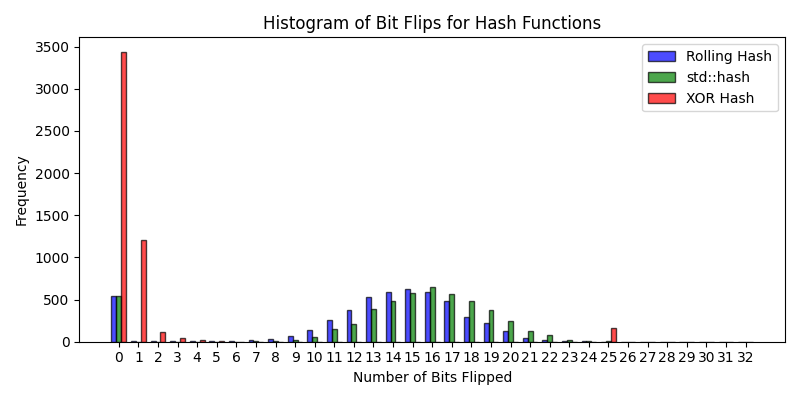
\includegraphics[width=0.7\linewidth]{grouped-histogram.png}
  \caption{No.\ of bits flipped on average by different hashing algorithms.}
\end{figure}

It is observed that among the given implementations, \texttt{std::hash} performs best, with the rolling hash close behind. \\
The nature of XOR hash and Random-Hash leads to poor performance on the avalanche test. \\
XOR hash performs poorly particularly because for the given algorithm, one bit flip in the input, implies one bit flip in the output.  

\begin{figure}[H]
  \centering
  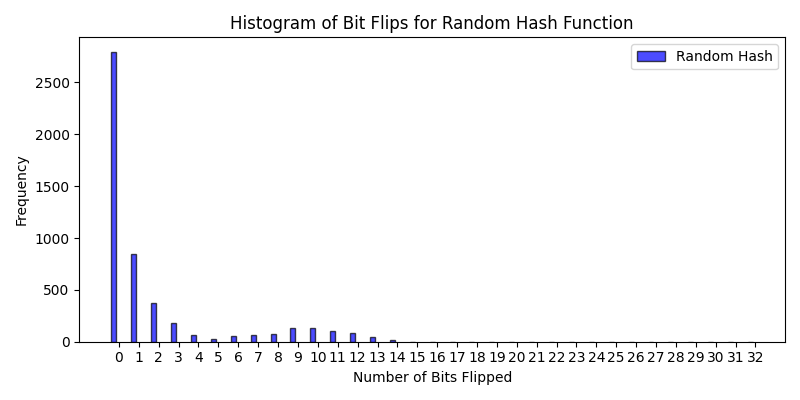
\includegraphics[width=0.7\linewidth]{random-hash-histogram.png}
  \caption{No.\ of bits flipped on average by the Random-Hash algorithm.}
\end{figure}

Random-Hash performs poorly because a flipped bit only affects the output if that bit is among the chosen bits for the mask (each chosen with probability 0.5), and because of the modulo distribution.

%====================================================
\section{Range Queries}\label{sec:range-queries-detail}

\subsection{Fenwick Trees (Binary Indexed Trees)\cite{fenwick_tree_cp}}
Given an array of integers, $A[0 \dots N-1]$, a Fenwick tree is just an array, $T[0 \dots N-1]$, where each element is equal to the sum of elements of $A$ in the range, $[g(i), i]$:  
$$T_i = \sum_{j = g(i)}^{i}{A_j}$$  
where
$$g(i) = i ~\&~ (i+1),$$
\begin{verbatim}
define sum(int r):
  res := 0
  while (r >= 0):
      res := res + t[r]
      r := g(r) - 1
  return res
\end{verbatim}
The above adds $[g(r), r]$, $[g(g(r) - 1), g(r) - 1]$, $\dots$, $[g(-1), -1]$ to the result.

\begin{verbatim}
define increase(int i, int delta):
  for all j with g(j) <= i <= j:
      t[j] := t[j] + delta
\end{verbatim}
Here jumps happen in the opposite direction; we need a way to iterate over all $j$'s, such that
$g(j) \le i \le j$.
We can find all such $j$'s by starting with $i$ and flipping the last unset bit. We will call this operation $h(j)$.
$$h(j) = j ~|~ (j+1)$$

Using this, we get the following:
\begin{verbatim}
define increase(int i, int delta):
  while (i < n):
    t[i] := t[i] + delta
    i = h(i)
\end{verbatim}

\begin{figure}[H]
  \centering
  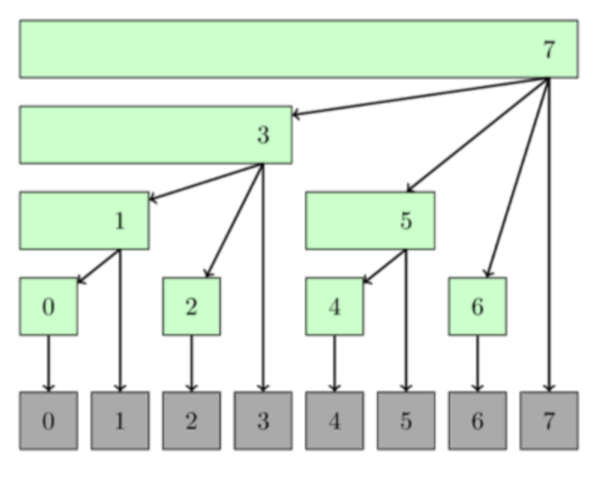
\includegraphics[width=0.7\linewidth]{fenwick.png}
  \caption{Nodes of a Fenwick tree and covered ranges.\cite{fenwick_tree_cp}}
\end{figure}

Time Complexity:
While a standard construction may take $\;O(n\log n)$ time, it is possible to do so in linear time.
\begin{itemize}
  \item Precompute: $\;O(n)$
  \item Query: $\;O(\log n)$
\end{itemize}

\subsection{Segment Trees\cite{segment_tree_cp}}
A Segment Tree stores information about array intervals in a tree, allowing efficient range queries and updates. \\
The idea is to create a binary tree, where the root covers aggregate over the entire range, leaf nodes only cover a single element and any internal node has two children, each covering half its range. \\
The above enforces logarithmic depth since at each level, ranges get halved. The logarithmic depth allows for logarithmic query times for both updation and interrogation. \\
This holds as at each level only $O(1)$ nodes are relevant to any query (since anything to the left/right of a range can be ignored for computation).

\begin{figure}[H]
  \centering
  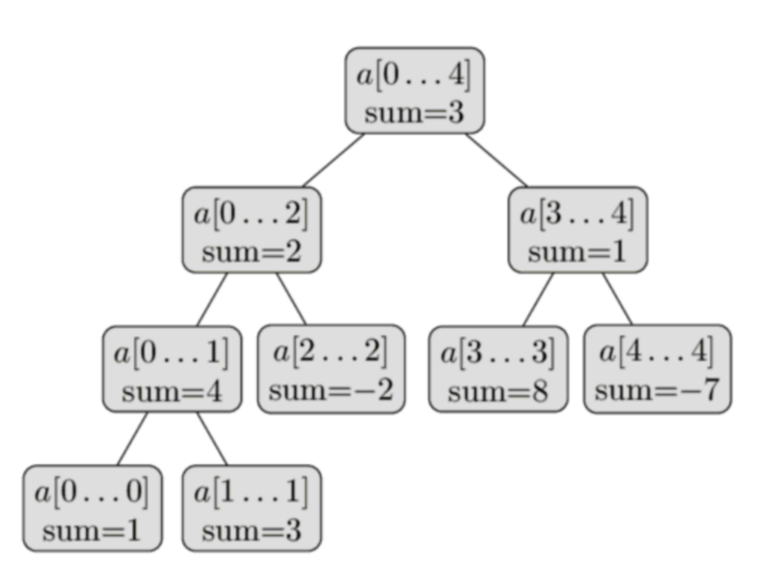
\includegraphics[width=0.7\linewidth]{segtree.png}
  \caption{Nodes of a Segment tree constructed over $[1, 3, -2, 8, -7]$.\cite{segment_tree_cp}}
\end{figure}

Time Complexity:
\begin{itemize}
  \item Precompute: $\;O(n)$
  \item Query: $\;O(\log n)$
\end{itemize}

The iterative variant\cite{iterative_segment_tree} of segment trees instead follows a bottom-up approach, where the tree is treated as an array and starting from the leaf-level, relevant nodes are visited only using a loop and index arithmetic.

\subsection{Results}
Refer to Section~\ref{sec:range-queries-benchmarks}.

\bigskip
\hrule height 1pt
\bigskip

%====================================================
\section{Range Queries Benchmarks}\label{sec:range-queries-benchmarks}

Each size is tested with 10 instances per algorithm (evenly split update/sum queries).

\textbf{Array length, query count categories:}
\begin{itemize}
  \item Small-1: 10–100, 10–100
  \item Small-2: 10–100, 100–1{,}000
  \item Medium-1: 1{,}000–10{,}000, 1{,}000–10{,}000
  \item Medium-2: 1{,}000–10{,}000, 10{,}000–100{,}000
  \item Large: 100{,}000–1{,}000{,}000, 100{,}000–1{,}000{,}000
\end{itemize}

\begin{table}[H]
  \centering
  \begin{tabular}{@{}lccc@{}}
    \toprule
               & \textbf{Fenwick Tree}   & \textbf{Segment Tree}    & \textbf{Iterative Seg.\ Tree} \\ \midrule
    Small-1   & (1{,}255, 3{,}454)      & (3{,}853, 10{,}065)      & (1{,}205, 4{,}383)           \\
    Small-2   & (2{,}357, 16{,}172)     & (6{,}359, 49{,}646)      & (3{,}123, 21{,}445)          \\
    Medium-1  & (29{,}236, 161{,}666)   & (126{,}403, 844{,}780)   & (44{,}588, 313{,}366)        \\
    Medium-2  & (430{,}298, 1{,}735{,}205) & (2{,}341{,}528, 10{,}133{,}545) & (843{,}497, 3{,}598{,}143) \\
    Large     & (8{,}258{,}384, 25{,}595{,}156) & (38{,}811{,}311, 173{,}135{,}398) & (11{,}716{,}570, 54{,}932{,}104) \\
    \bottomrule
  \end{tabular}
  \caption{Least and highest execution times (in nanoseconds) across inputs.}
\end{table}

\begin{figure}[H]
  \centering
  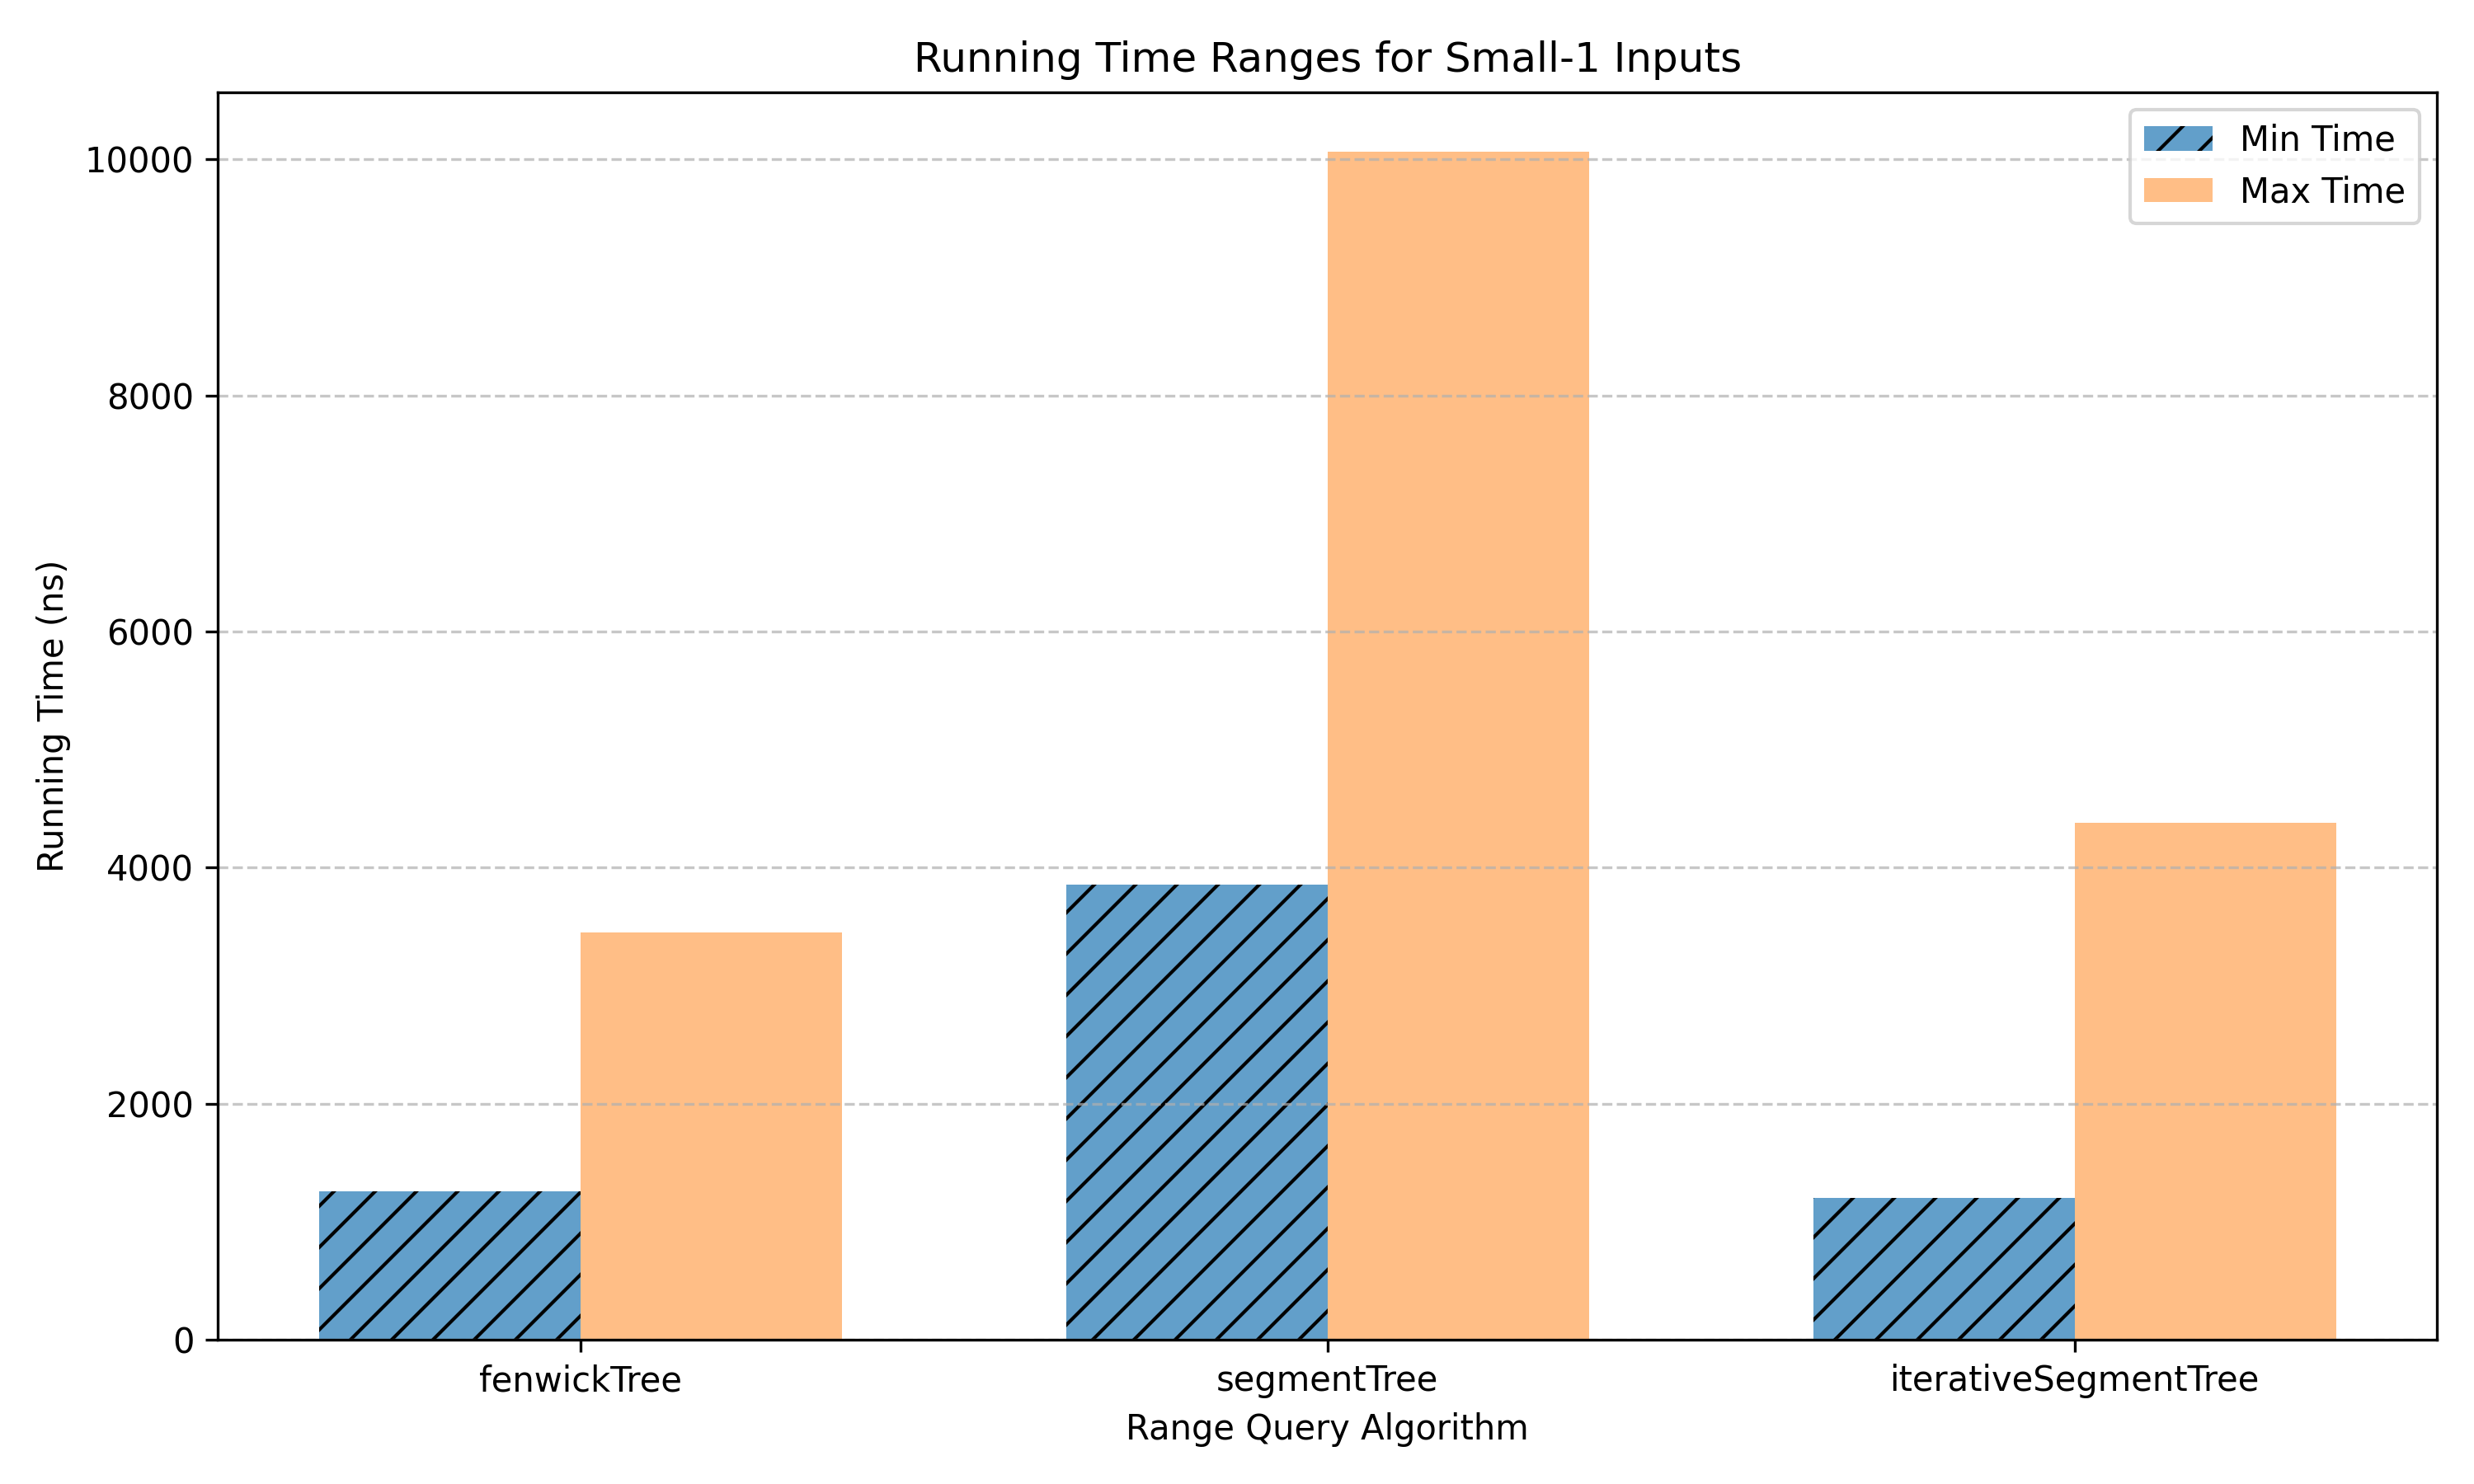
\includegraphics[width=0.45\linewidth]{range-queries-stats-small-1.png}
  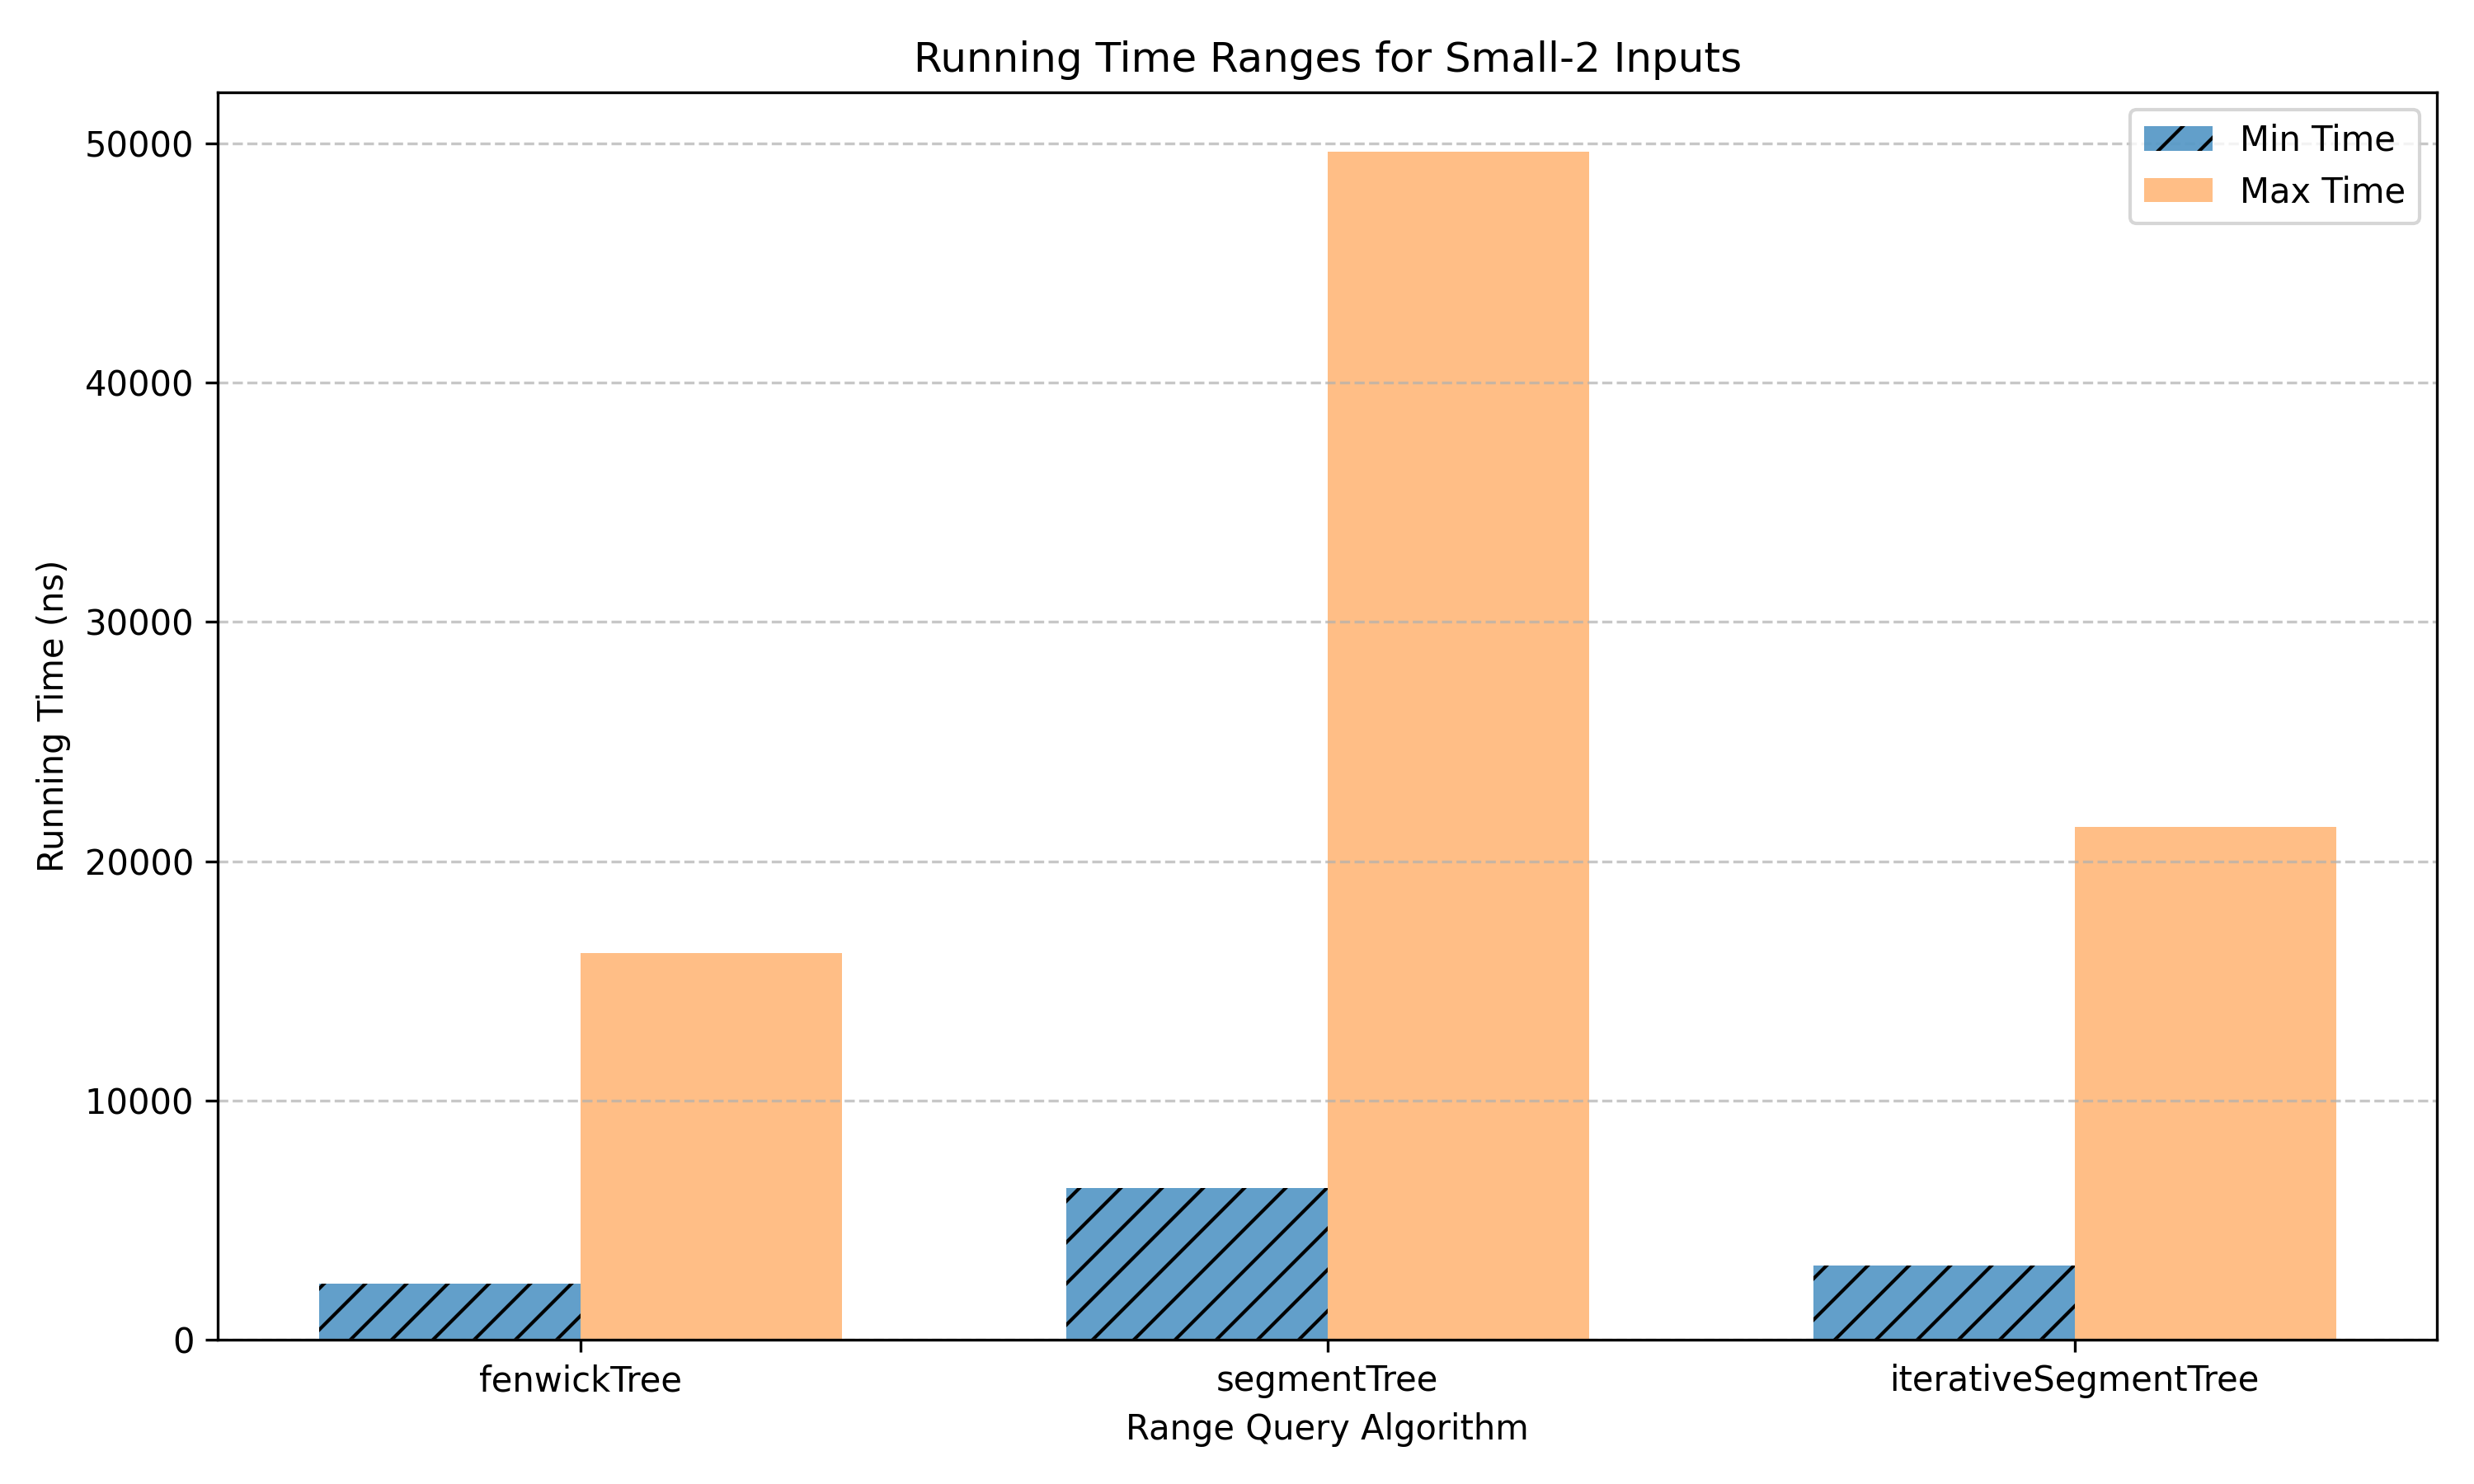
\includegraphics[width=0.45\linewidth]{range-queries-stats-small-2.png}
  \caption{Top: Small-1 (few queries) \& Small-2 (many queries).}
\end{figure}

\begin{figure}[H]
  \centering
  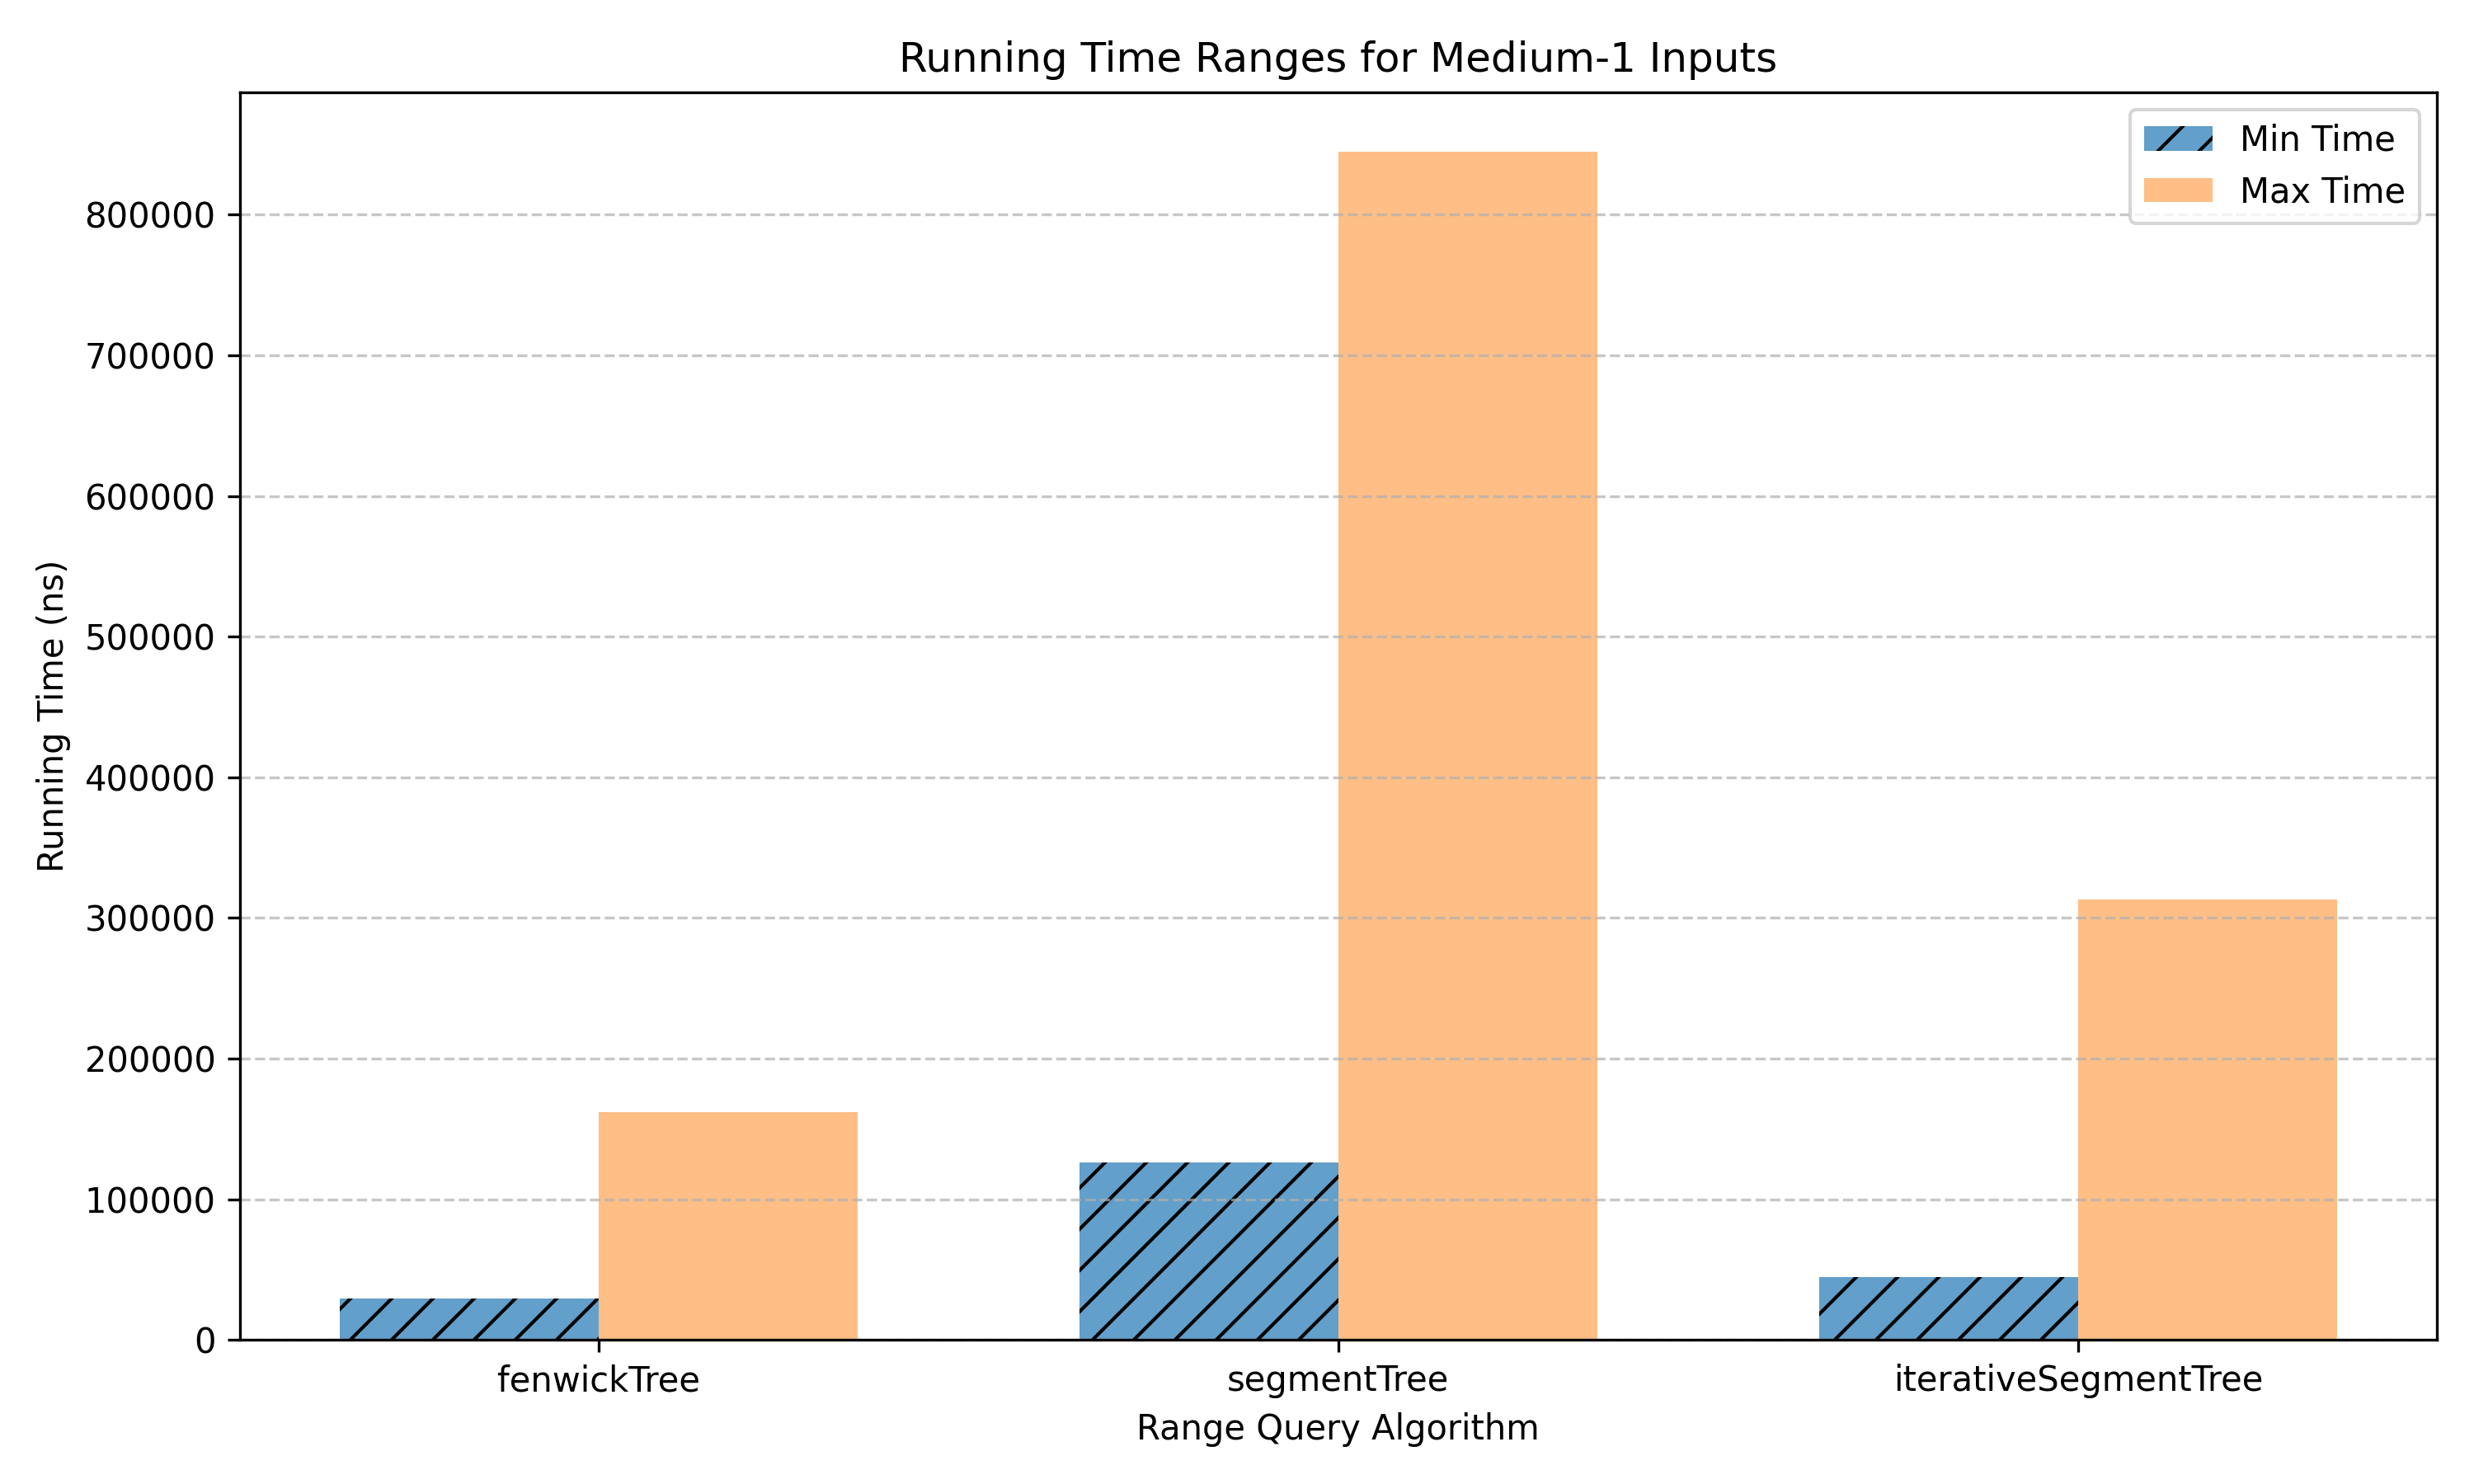
\includegraphics[width=0.45\linewidth]{range-queries-stats-medium-1.png}
  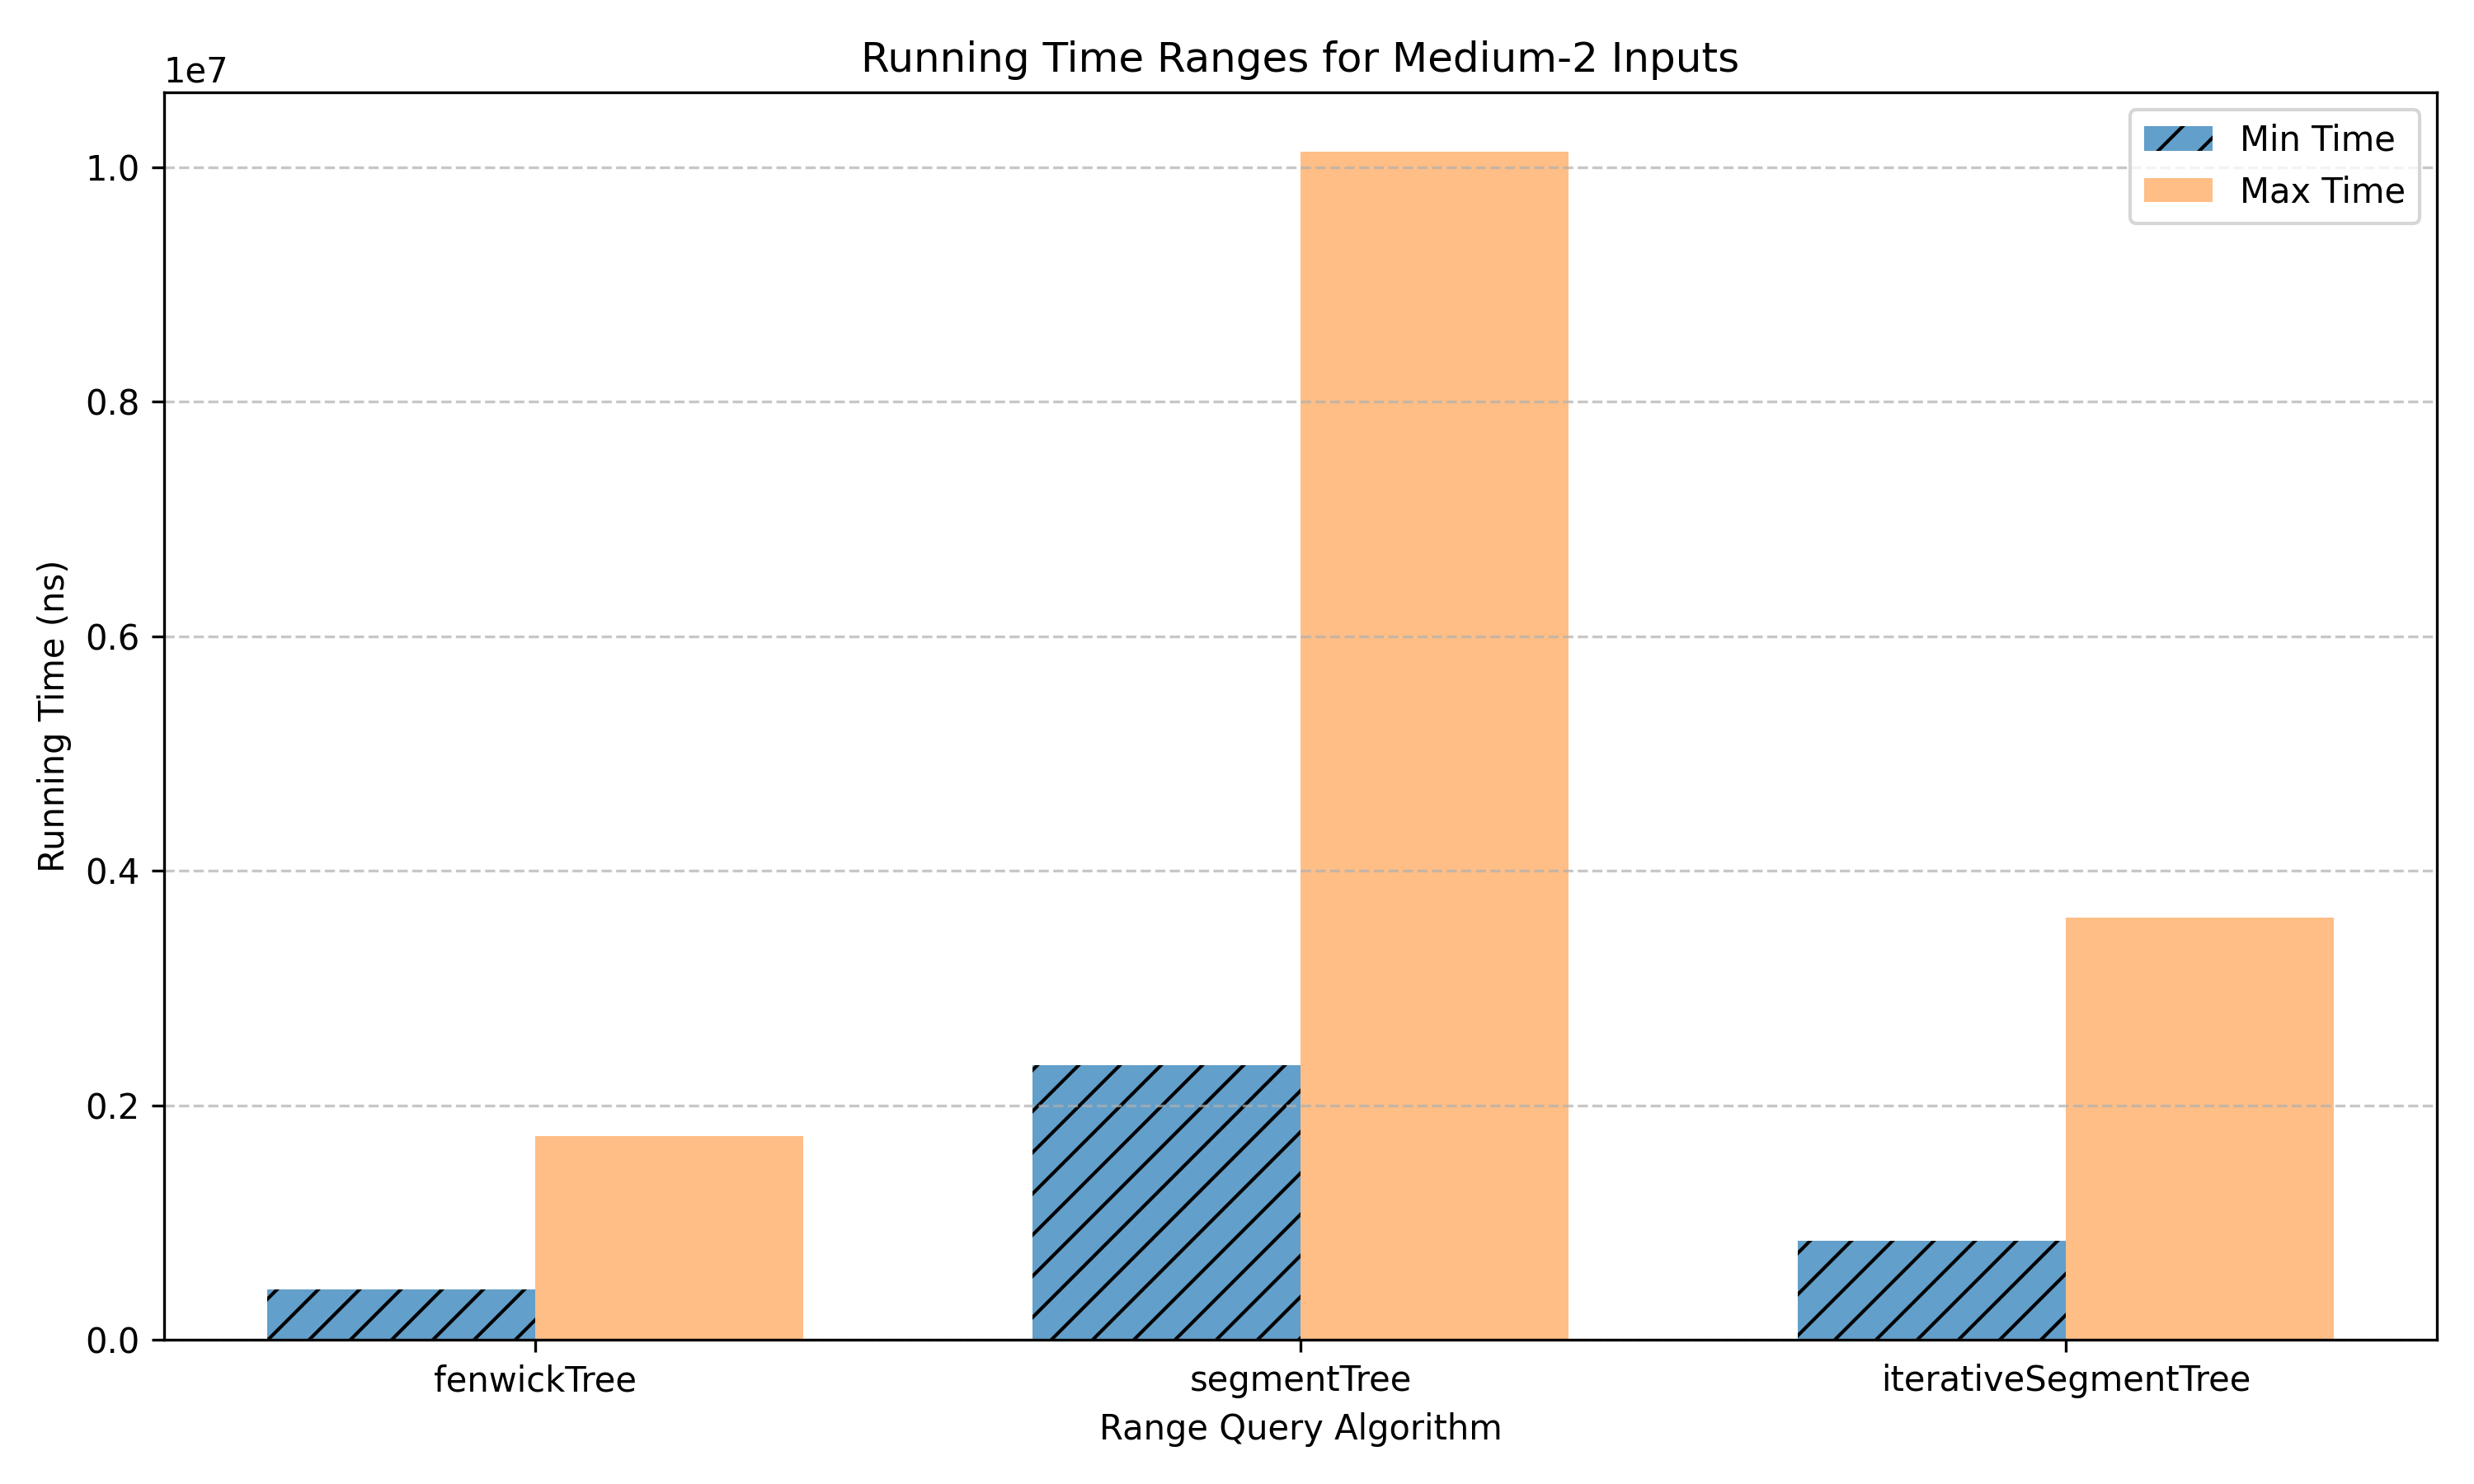
\includegraphics[width=0.45\linewidth]{range-queries-stats-medium-2.png}
  \caption{Medium-1 (few queries) \& Medium-2 (many queries).}
\end{figure}

\begin{figure}[H]
  \centering
  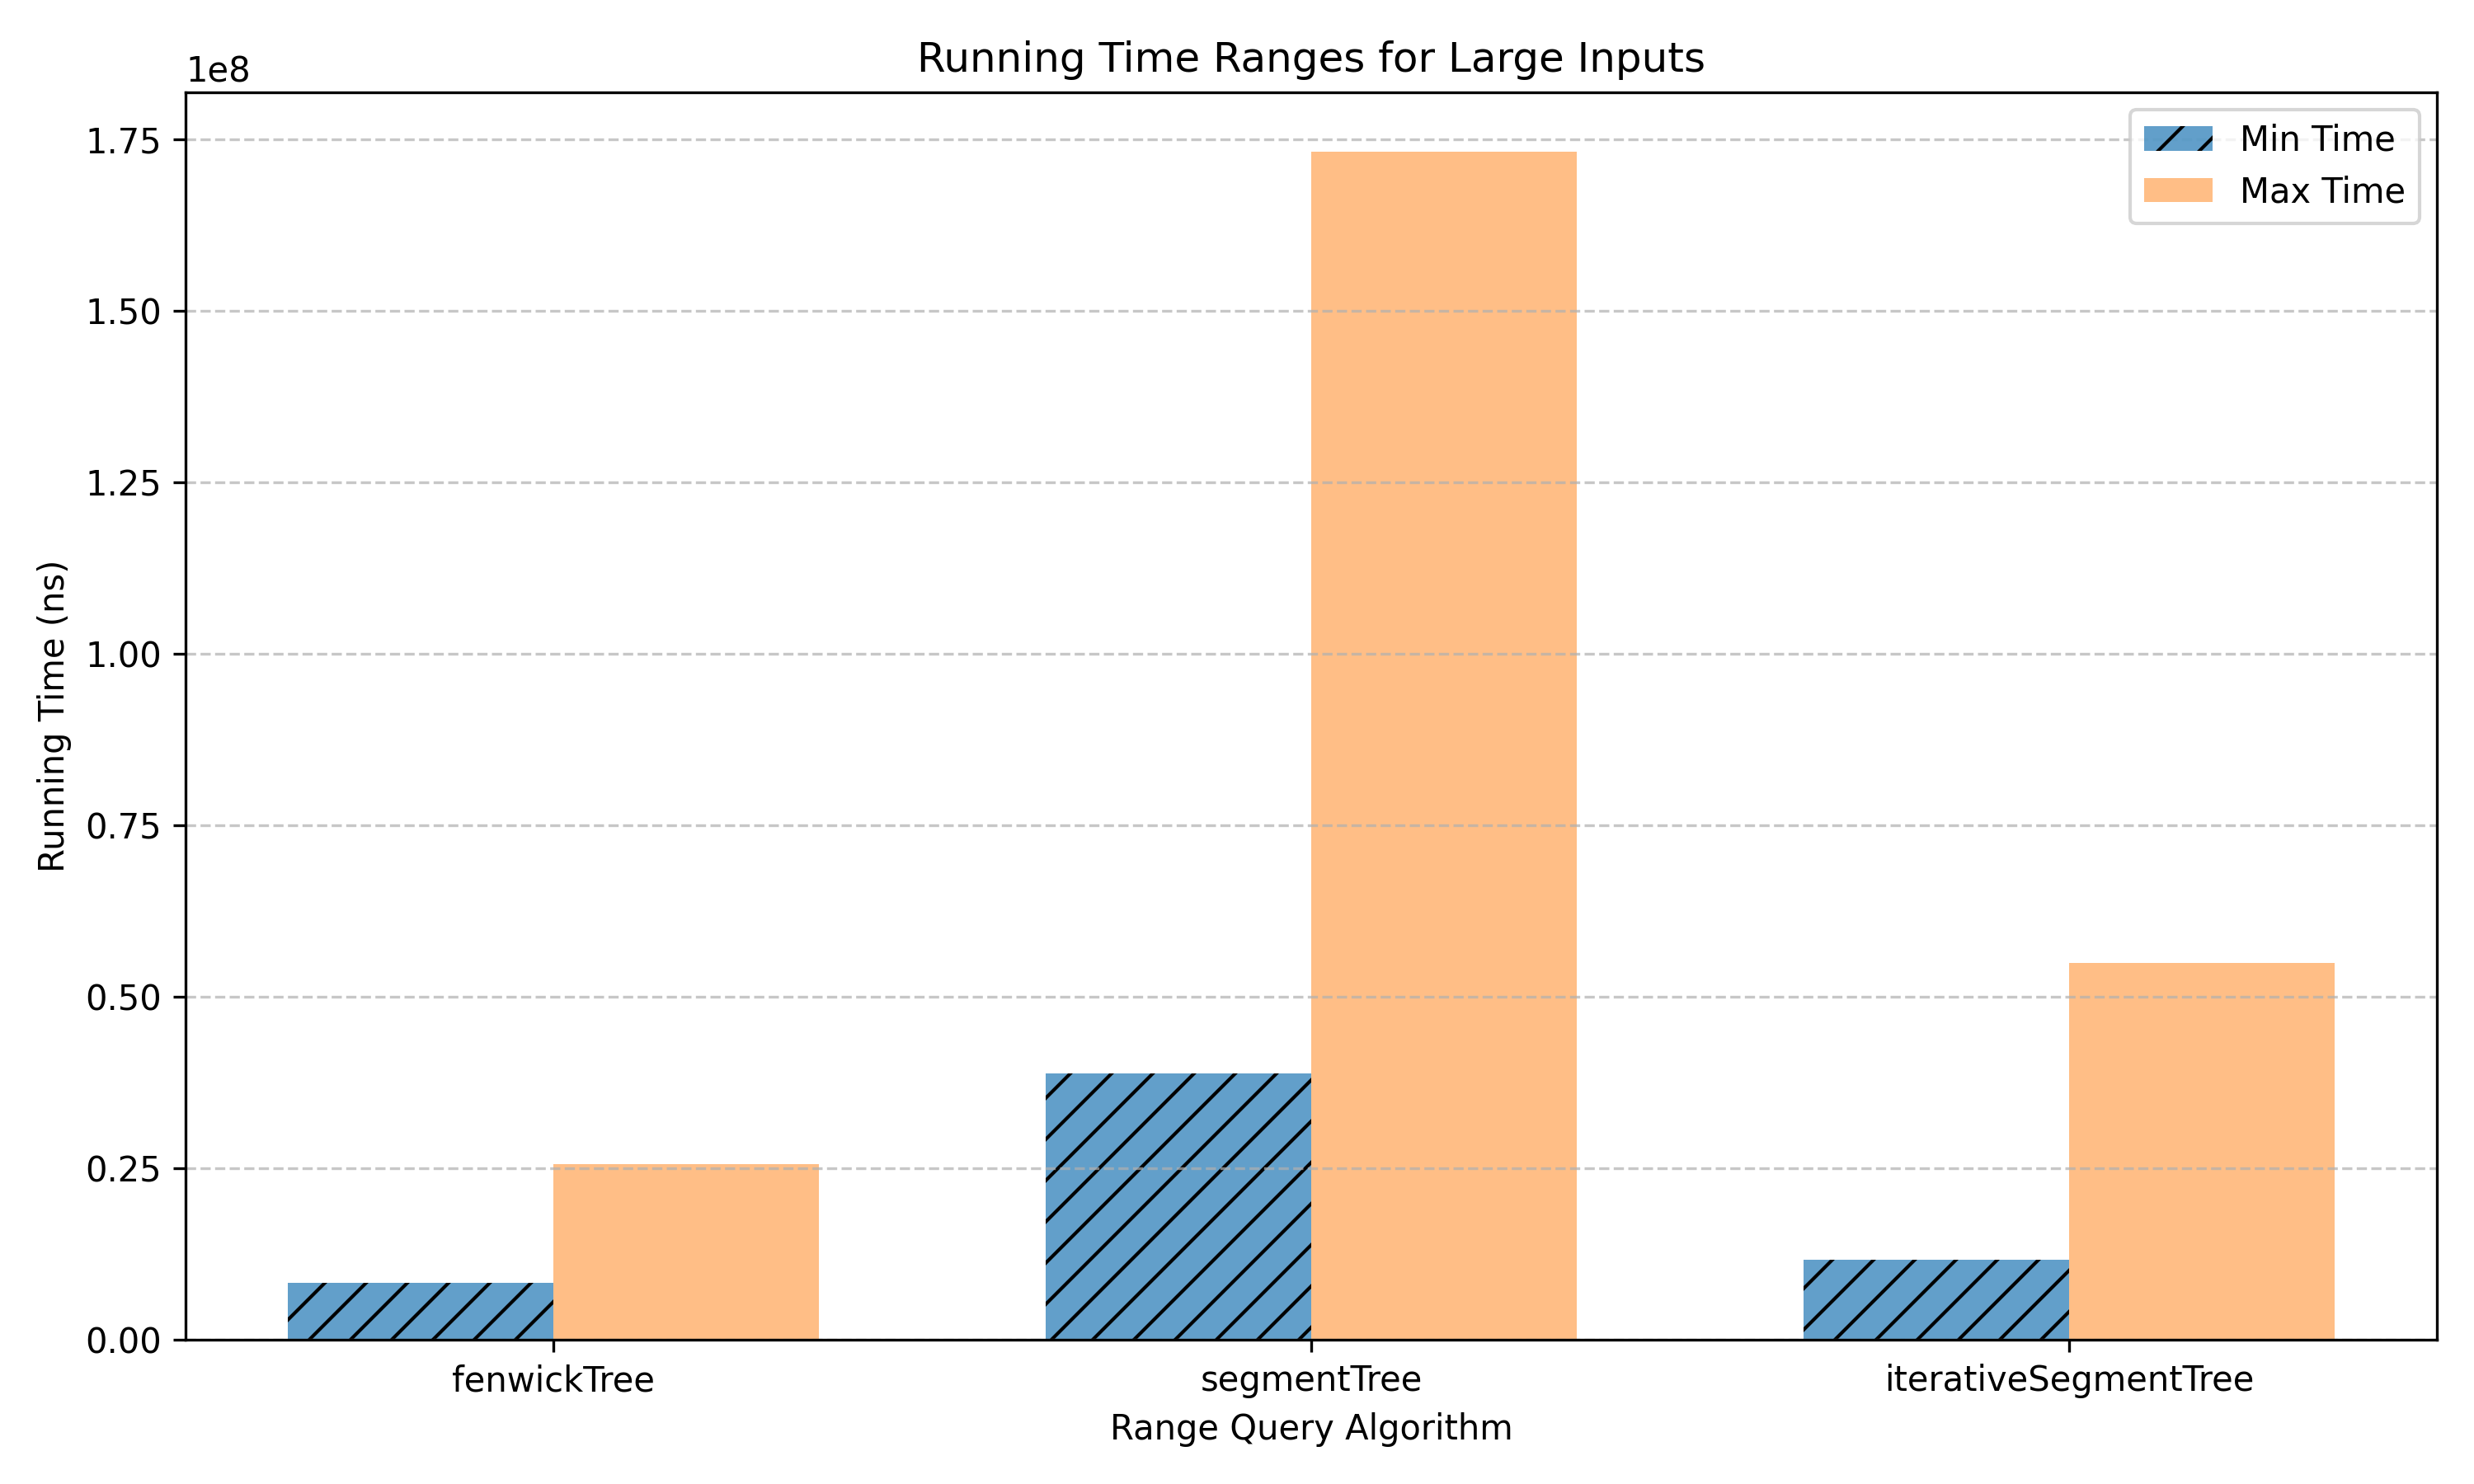
\includegraphics[width=0.7\linewidth]{range-queries-stats-large.png}
  \caption{Large inputs.}
\end{figure}

It is observed that across array sizes and query counts, fenwick trees typically perform best among the three, with the iterative version of segment tree following it closely, and the recursive segment tree lagging behind.  
In practice, the versatility of segment trees brings them to use above fenwick trees. For instance, even to handle range minimum queries, the standard fenwick trees fail, and we must use two in conjunction.\cite{fenwick_tree_rmq}


%====================================================
\section{Sorting}\label{sec:sorting-detail}

\subsection{Insertion Sort\cite{insertion_sort_wiki}}
Standard insertion sort with $O(n^2)$ running time for an $n$ length array.
\begin{verbatim}
i ← 1
while i < length(A)
    j ← i
    while j > 0 and A[j-1] > A[j]
        swap A[j] and A[j-1]
        j ← j - 1
    end while
    i ← i + 1
end while
\end{verbatim}

\subsection{Merge Sort\cite{merge_sort_wiki}}
Standard merge sort with $O(n\log n)$ running time for an $n$ length array.
\begin{verbatim}
define merge_sort(m):
    if length(m) <= 1 then return m
    split m into left/right halves
    left  := merge_sort(left)
    right := merge_sort(right)
    return merge(left, right)
\end{verbatim}

\begin{verbatim}
define merge(left, right):
  var result := empty list

  while left is not empty and right is not empty do
    if first(left) <= first(right) then
      append first(left) to result
      left := rest(left)
    else
      append first(right) to result
      right := rest(right)

  while left is not empty do
    append first(left) to result
    left := rest(left)

  while right is not empty do
    append first(right) to result
    right := rest(right)
\end{verbatim}

\subsection{QuickSort\cite{quicksort_wiki}}
Standard quick sort using random-pivot with worst case $O(n^2)$ and average case $O(n\log n)$ running time for an $n$ length array.
\begin{verbatim}
define quicksort(A, lo, hi):
    if lo >= hi then return
    p := partition(A, lo, hi)
    quicksort(A, lo, p-1)
    quicksort(A, p+1, hi)
\end{verbatim}
\begin{verbatim}
define partition(A, lo, hi):
  pivot_idx = random(lo, hi)
  swap A[pivot_idx] and A[hi]
  pivot := A[hi]
  i := lo

  for j := lo to hi - 1 do 
    if A[j] <= pivot then 
      swap A[i] with A[j]
      i := i + 1

  swap A[i] with A[hi]
  return i
\end{verbatim}

\subsection{Hybrid Sort}
While a variety of hybrid sorting algorithms exist, we study a mix of quicksort and insertion sort for its practical efficiency.  \\
A mix of the quick-sort above and insertion sort, with $INSERTION\_SORT\_LIMIT = 65$.\cite{dual_pivot_quicksort_jdk}  \\
A subarray $s$ of length $slen$ is sorted using insertion sort if $slen \leq INSERTION\_SORT\_LIMIT$. Otherwise, the mechanics of quick sort as above are applied. \\
Algorithm runs with worst case $O(n^2)$ and average case $O(n\log n)$ running time for an $n$ length array. \\
Faster in practice considering the practical improvements through insertion sort's efficiency over small subarrays.  \\
Other noteworthy hybrids:
\begin{itemize}
  \item {Merge Sort + Insertion Sort} \\
  Same as above, applying insertion sort on small subarrays.  
  An interesting variant of the same can be found under \hyperref[https://en.wikipedia.org/wiki/Timsort]{Timsort}. 
  \item {QuickSort + HeapSort} \\
  This algorithm applies quicksort till a recursive-depth of $O(\log n)$ for an $n$ length array, and switches to heapsort thereafter if still unsorted.  
  Doing so allows the algorithm to guarantee worst case $O(n\log n)$ running time while benefitting from general efficiency of quicksort.
\end{itemize}

\subsection{Results}
Refer to Section~\ref{sec:sorting-benchmarks}.

\bigskip
\hrule height 1pt
\bigskip

%====================================================
\section{Sorting Benchmarks}\label{sec:sorting-benchmarks}

Tested on 10 instances per algorithm in three size categories:

\begin{itemize}
  \item Small: 10–200
  \item Medium: 1{,}000–20{,}000
  \item Large: 100{,}000–2{,}000{,}000
\end{itemize}

\begin{table}[H]
  \centering
  \setlength{\tabcolsep}{0.5pt}
  \begin{tabular}{lcccc}
    \toprule
      & InsertionSort     & QuickSort             & MergeSort            & HybridSort           \\ \midrule
    Small  & (709, 7{,}473)       & (768, 6{,}078)         & (933, 7{,}776)        & (763, 6{,}022)        \\
    Medium & (141{,}312, 10{,}548{,}489) & (81{,}225, 880{,}327)  & (94{,}431, 1{,}043{,}705) & (72{,}792, 769{,}667) \\
    Large  & (NA, NA)            & (9{,}733{,}001, 98{,}435{,}984) & (11{,}691{,}272, 120{,}194{,}603) & (8{,}779{,}871, 90{,}966{,}402) \\ 
    \bottomrule
  \end{tabular}
  \caption{Sorting algorithms: least and highest times (nanoseconds).}
\end{table}

\begin{figure}[H]
  \centering
  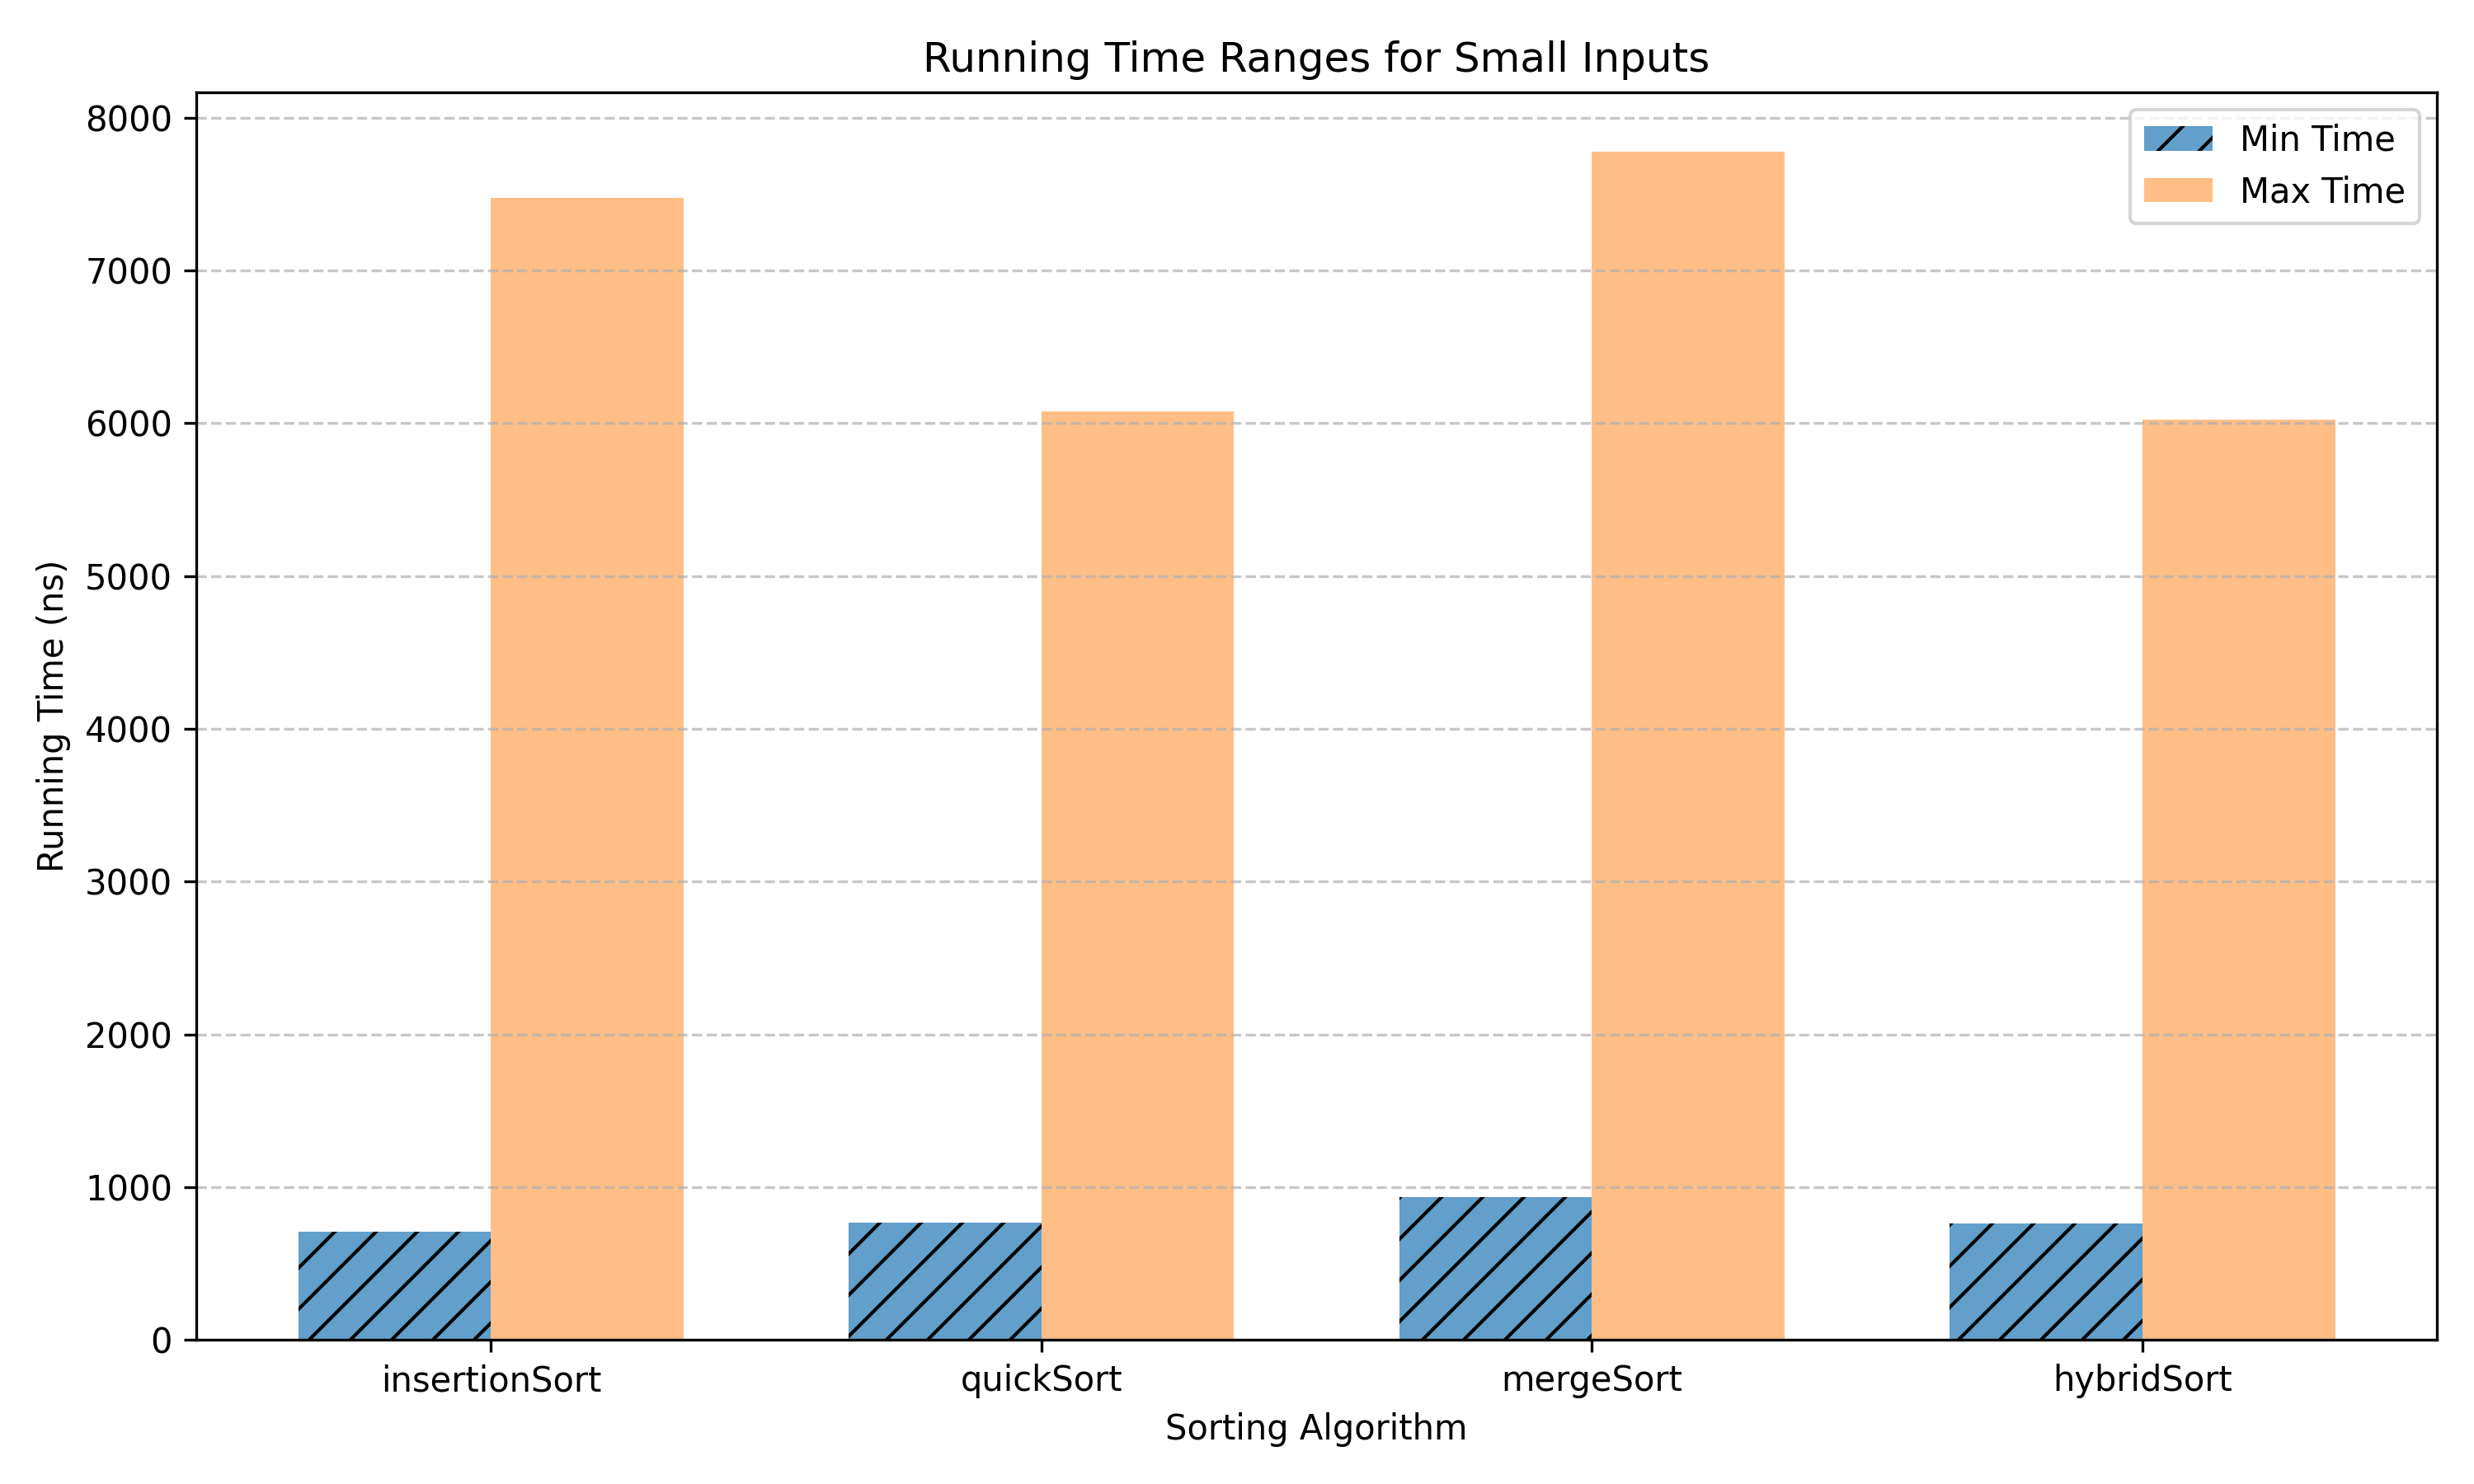
\includegraphics[width=0.7\linewidth]{sorting-stats-small.png}
  \caption{Least and highest running times on small inputs.}
\end{figure}

\begin{figure}[H]
  \centering
  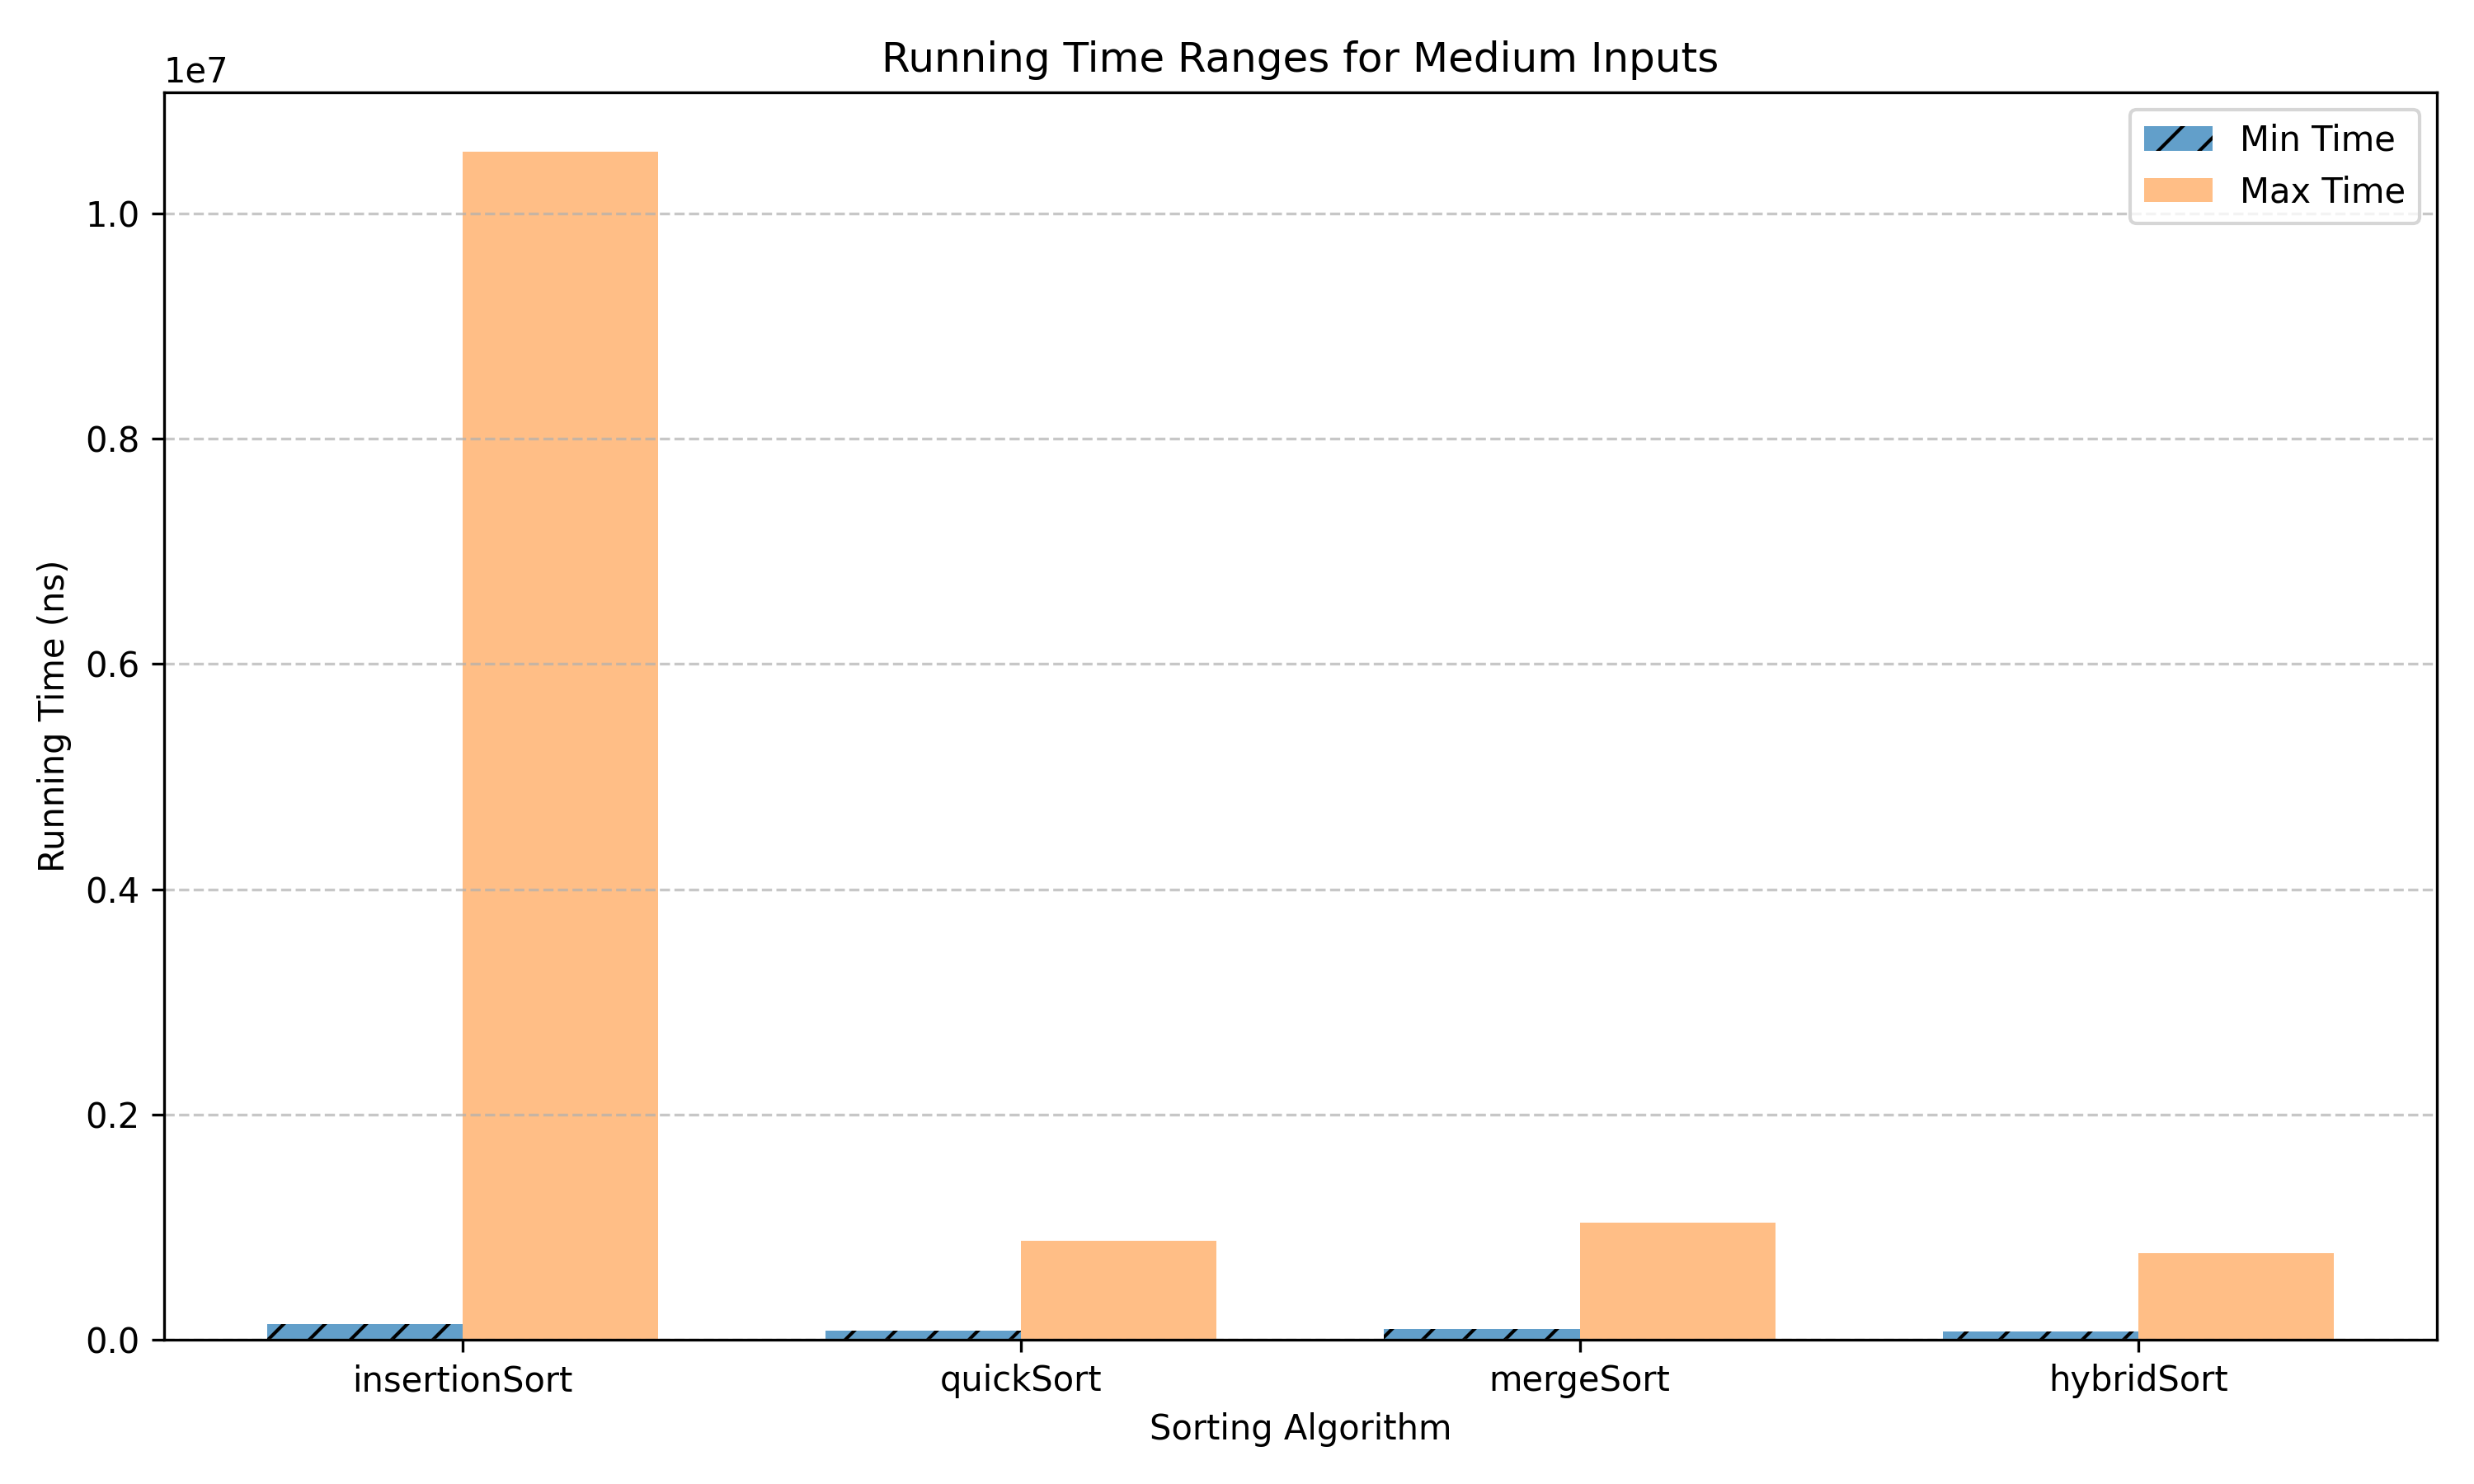
\includegraphics[width=0.7\linewidth]{sorting-stats-medium.png}
  \caption{Least and highest running times on medium sized inputs.}
\end{figure}

\begin{figure}[H]
  \centering
  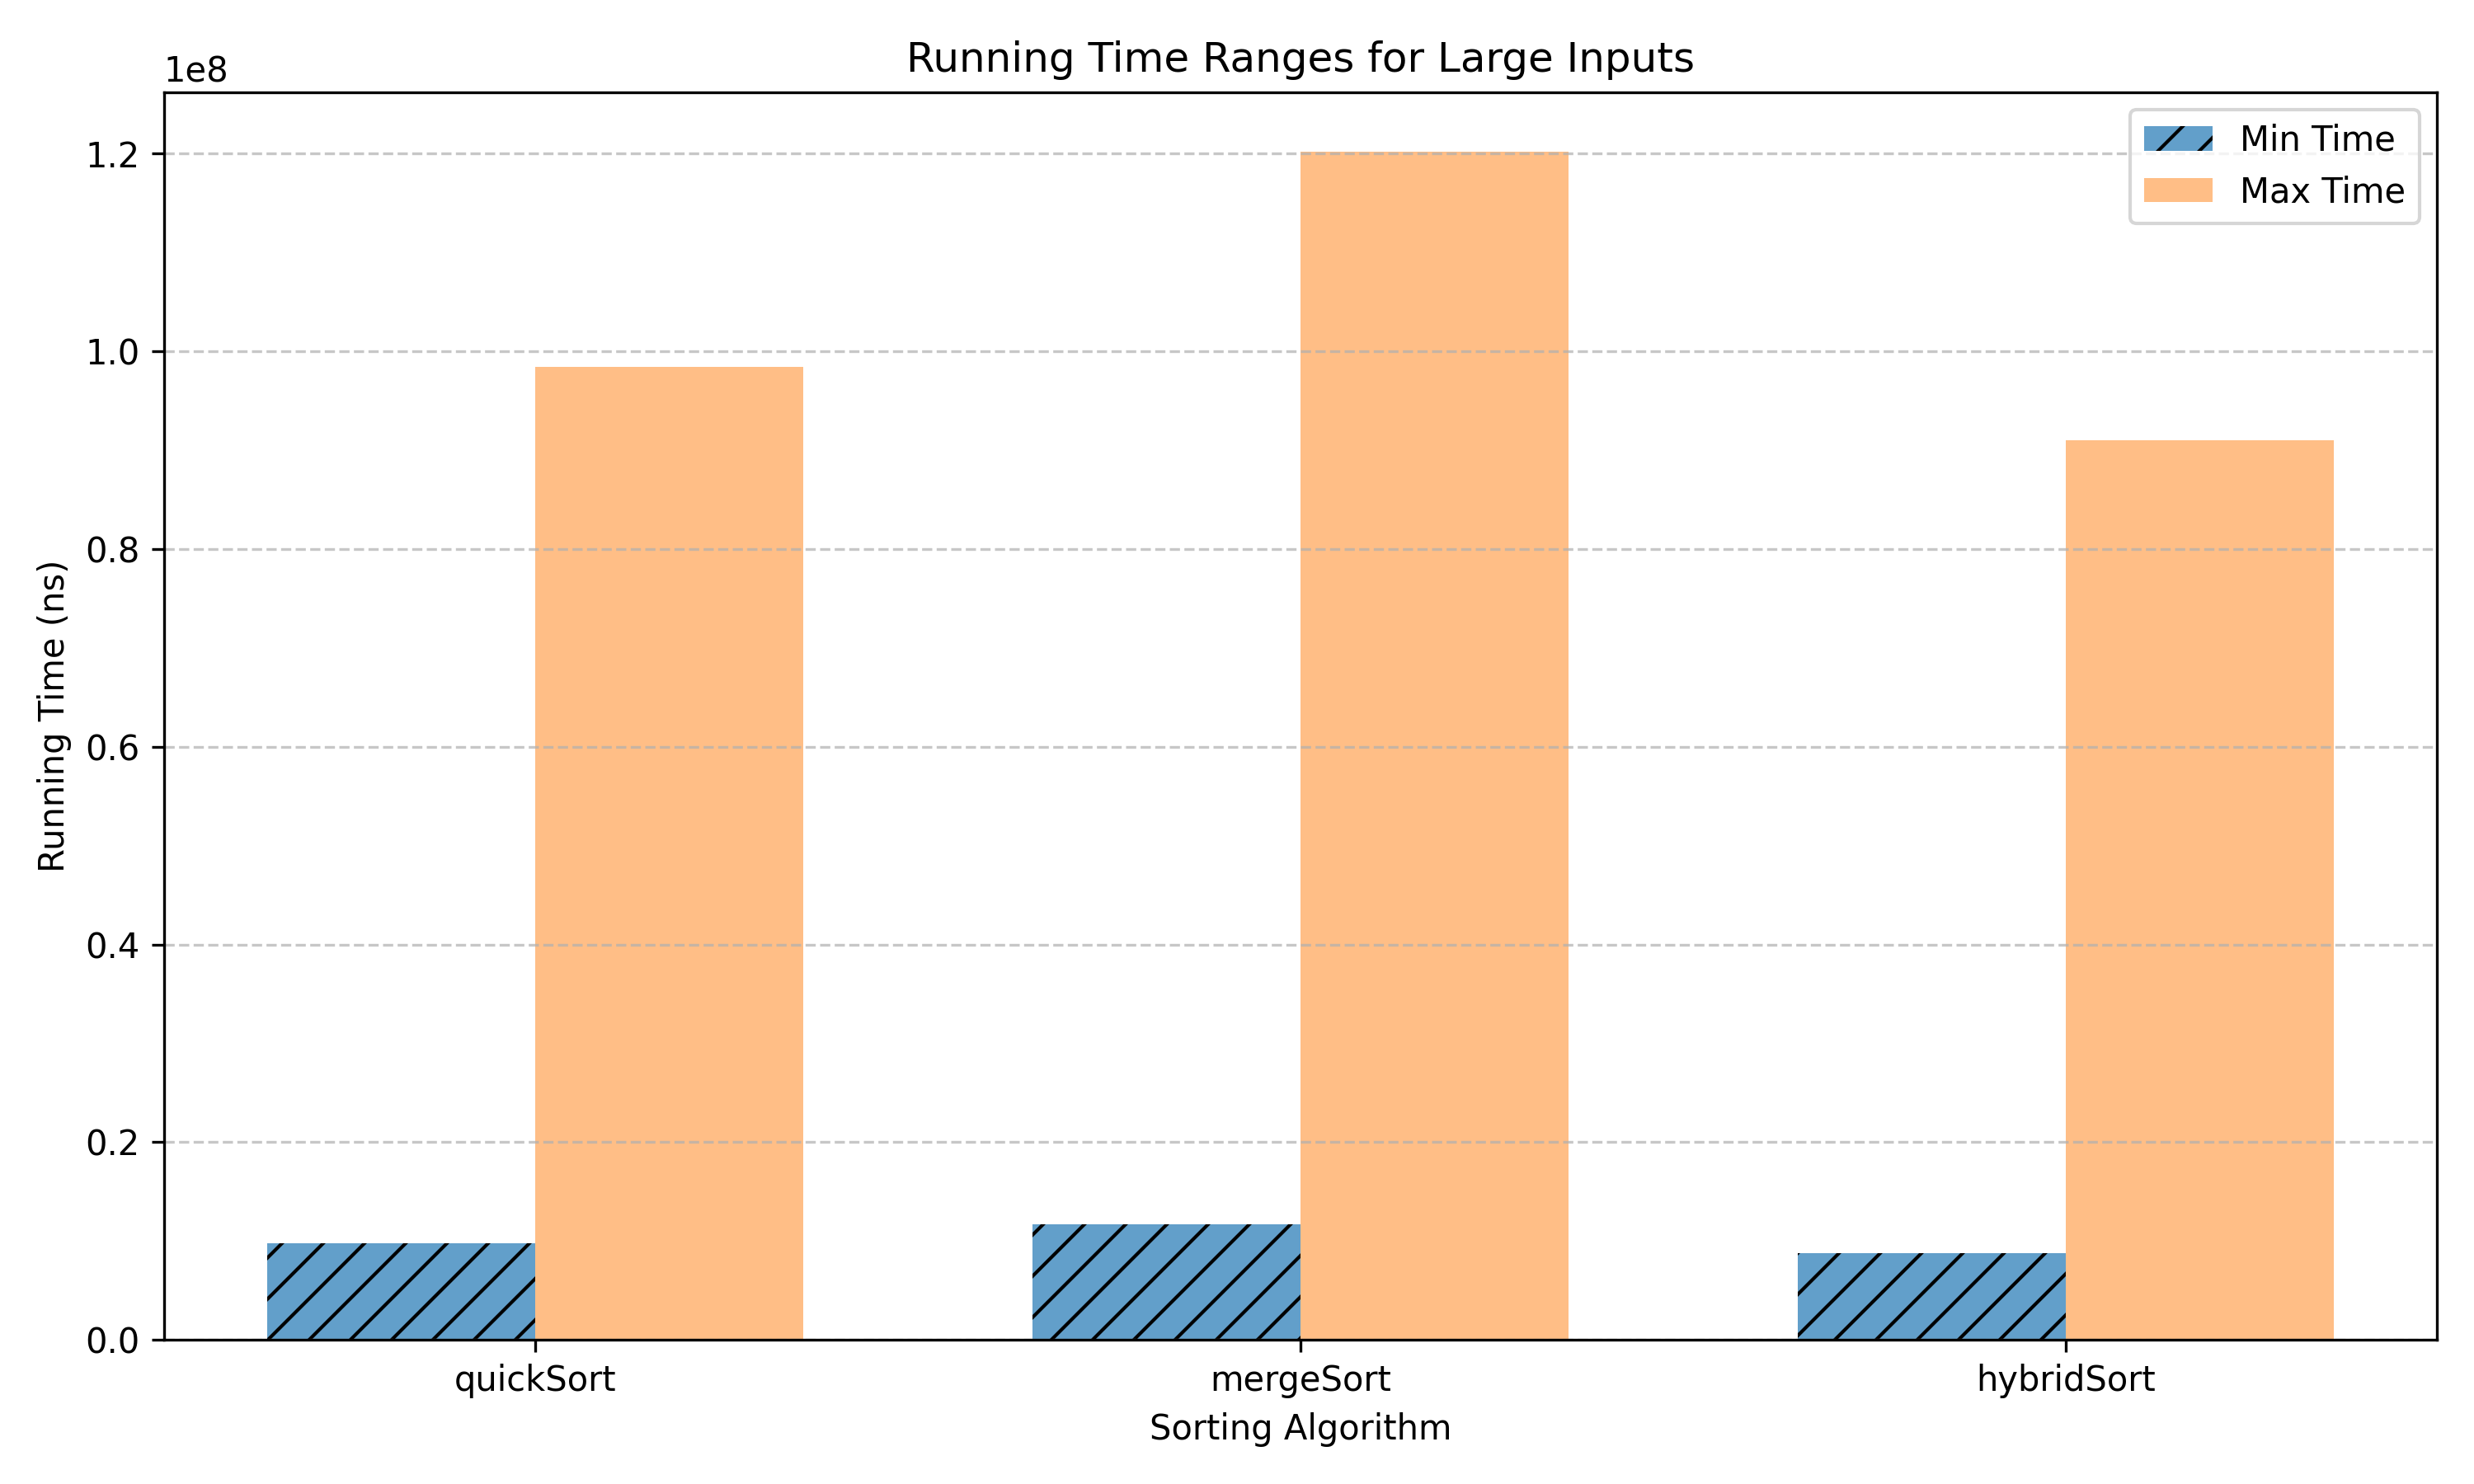
\includegraphics[width=0.7\linewidth]{sorting-stats-large.png}
  \caption{Least and highest running times on large inputs.}
\end{figure}

It is observed that for small inputs, InsertionSort is typically fast in practice, by virtue of its reliance on the same, HybridSort performs similarly, QuickSort lags behind a little and MergeSort is slightly slower still. \\
In comparison, for medium to large sized inputs, InsertionSort expectedly blows up (since it is quadratic in time complexity) and HybridSort performs best, QuickSort lags behind a little and MergeSort is slightly slower still.

%====================================================
\section{Strings}\label{sec:strings-detail}

\subsection{KMP\cite{kmp_cp}}
The KMP algorithm, named after Knuth, Morris, and Pratt, is an efficient implementation of the prefix function. \\
Given a string $s$, of length $n$, the prefix function is defined as an array $p$ of length $n$, where $p[i]$ is the length of the longest proper prefix of the substring $s[0 \dots i]$ which is also a suffix of this substring.
A proper prefix of a string is a prefix that is not equal to the string itself. By definition, $p[0] = 0$. \\
Mathematically, $p[i] = max(k : s[0 \dots k-1] = s[i - (k - 1)..i])$, $k = 0 \dots i$  \\
While a trivial implementation runs in $O(n^2)$ time, KMP runs in $O(n)$ time. \\
An obvious observation is that the values of the prefix function can only increase by 1 between neighbouring indices. \\
Secondly, if $s[i + 1] = s[p[i]]$, $p[i + 1] = p[i] + 1$. \\
Next, we can use the fact that $s[p[i]+1:i] = s[0:p[i]-1]$ and find the largest prefix matching thus far, by looking at the value of p for the prefix as it is equivalent to the current substring. \\
This process is repeated until either the substring can be extended to match a prefix or there is no match. \\
From the above, since there can be at most $n$ increments to the prefix value, and an increment/decrement takes $O(1)$ time, the running time is bounded by $O(n)$.

Applications:
\begin{itemize}
 \item Search for a substring in a string
 \item Counting the number of occurrences of each prefix
 \item Compressing a string - representing a string $s$ as $t+ \dots +t$ for some prefix $t$ with the shortest length.
\end{itemize}

\subsection{Manacher\cite{manacher_cp}}
Manacher's algorithm provides an efficient way to find all sub-palindromes in a string $s$ of length $n$ in $O(n)$ time. \\
Formally, given a string $s$ with length $n$, it finds all the pairs $(i, j)$ such that substring $s[i \dots j]$ is a palindrome.
Note that while there may be upto $n^2$ such substrings, we can instead store their information succintly, only keeping the following:
\begin{itemize}
  \item for odd length palindromes, store for the central character, the length of the largest palindromic substring
  \item for even length palindromes, store for the central gap, the length of the longest palindromic substring
\end{itemize}
By only storing the longest around the center, we know all others as well since for any palindrome $p$ of length $k$, $p[1 \dots k - 2]$ ($0$ indexed) is also a palindrome. \\
The algorithm stores the right-most found subpalindrome $(l, r)$. Since we know that $(l, r)$ is a palindrome, we can find the mirror position of substrings within to check for extension with the current character.

Applications:
\begin{itemize}
  \item Find largest subpalindrome
  \item Count no. of subpalindromes
\end{itemize}

\subsection{Rabin-Karp\cite{rabin_karp_cp}}
Based on the idea of \hyperref[sec:hashing-algos-considered]{hashing}, the Rabin-Karp algorithm compares the hash of substrings of a text $t$ to that of a pattern $p$.  
The efficient implementation assumes that a matching hash implies (with high confidence) that the substring matches the pattern.  \\
The hash of a substring can be computed by substring $s[i \dots j]$ can be found as follows:
$$hs_{ij} = (h[0 \dots j] - h[0 \dots i - 1]) \cdot 2^{n - (j - i)} \bmod m$$
Where $n$ is the length of the whole string. We multiply by the power of two to normalize hashes across differently positioned substrings.
In practice, results from our tests agree that the algorithm rarely fails (with good hash functions).  
It did not fail over a single instance among $100+$ test runs.

Applications:
\begin{itemize}
 \item Search for a substring in a string
 \item Counting the number of different substrings
 \item With binary search - count no. of subpalindromes/find largest subpalindrome
\end{itemize}

\subsection{Z-Function\cite{z_function_cp}}
The Z-function calculates for each $i$, the greatest number of characters starting from the position $i$ that coincide with the first characters of $s$.  
In other words, $z[i]$ is the length of the longest string that is, at the same time, a prefix of $s$ and a prefix of the suffix of $s$ starting at $i$.  \\
The idea is to store the right-most prefix-match found, $[l, r)$. If the current index is outside this, we run the trivial algorithm, otherwise, similar to KMP, we can re-use already computed prefix information.

Applications:
\begin{itemize}
 \item Search for a substring in a string
 \item Counting the number of occurrences of each prefix
 \item Compressing a string - representing a string $s$ as $t+ \dots +t$ for some prefix $t$ with the shortest length.
\end{itemize}

\subsection{Results}
Refer to Section~\ref{sec:strings-benchmarks}.

\bigskip
\hrule height 1pt
\bigskip

%====================================================
\section{Strings Benchmarks}\label{sec:strings-benchmarks}

Tested 100 instances per algorithm in sizes Small (200–400), Medium (2{,}000–4{,}000), Large (20{,}000–40{,}000), Huge (200{,}000–400{,}000).

\begin{table}[H]
  \centering
  \begin{tabular}{@{}lccc@{}}
    \toprule
    Size   & Rabin–Karp            & KMP                  & Z-Function            \\ \midrule
    Small  & (1{,}636, 45{,}676)   & (601, 4{,}348)       & (657, 5{,}191)        \\
    Medium & (13{,}937, 102{,}892) & (2{,}548, 23{,}085)  & (3{,}598, 25{,}824)   \\
    Large  & (148{,}434, 764{,}632)& (24{,}126, 206{,}257)& (37{,}017, 225{,}779) \\
    Huge   & (1{,}557{,}756, 4{,}086{,}762) & (244{,}870, 1{,}547{,}581) & (324{,}337, 1{,}749{,}875) \\
    \bottomrule
  \end{tabular}
  \caption{Least and highest pattern matching times (nanoseconds).}
\end{table}

\begin{figure}[H]
  \centering
  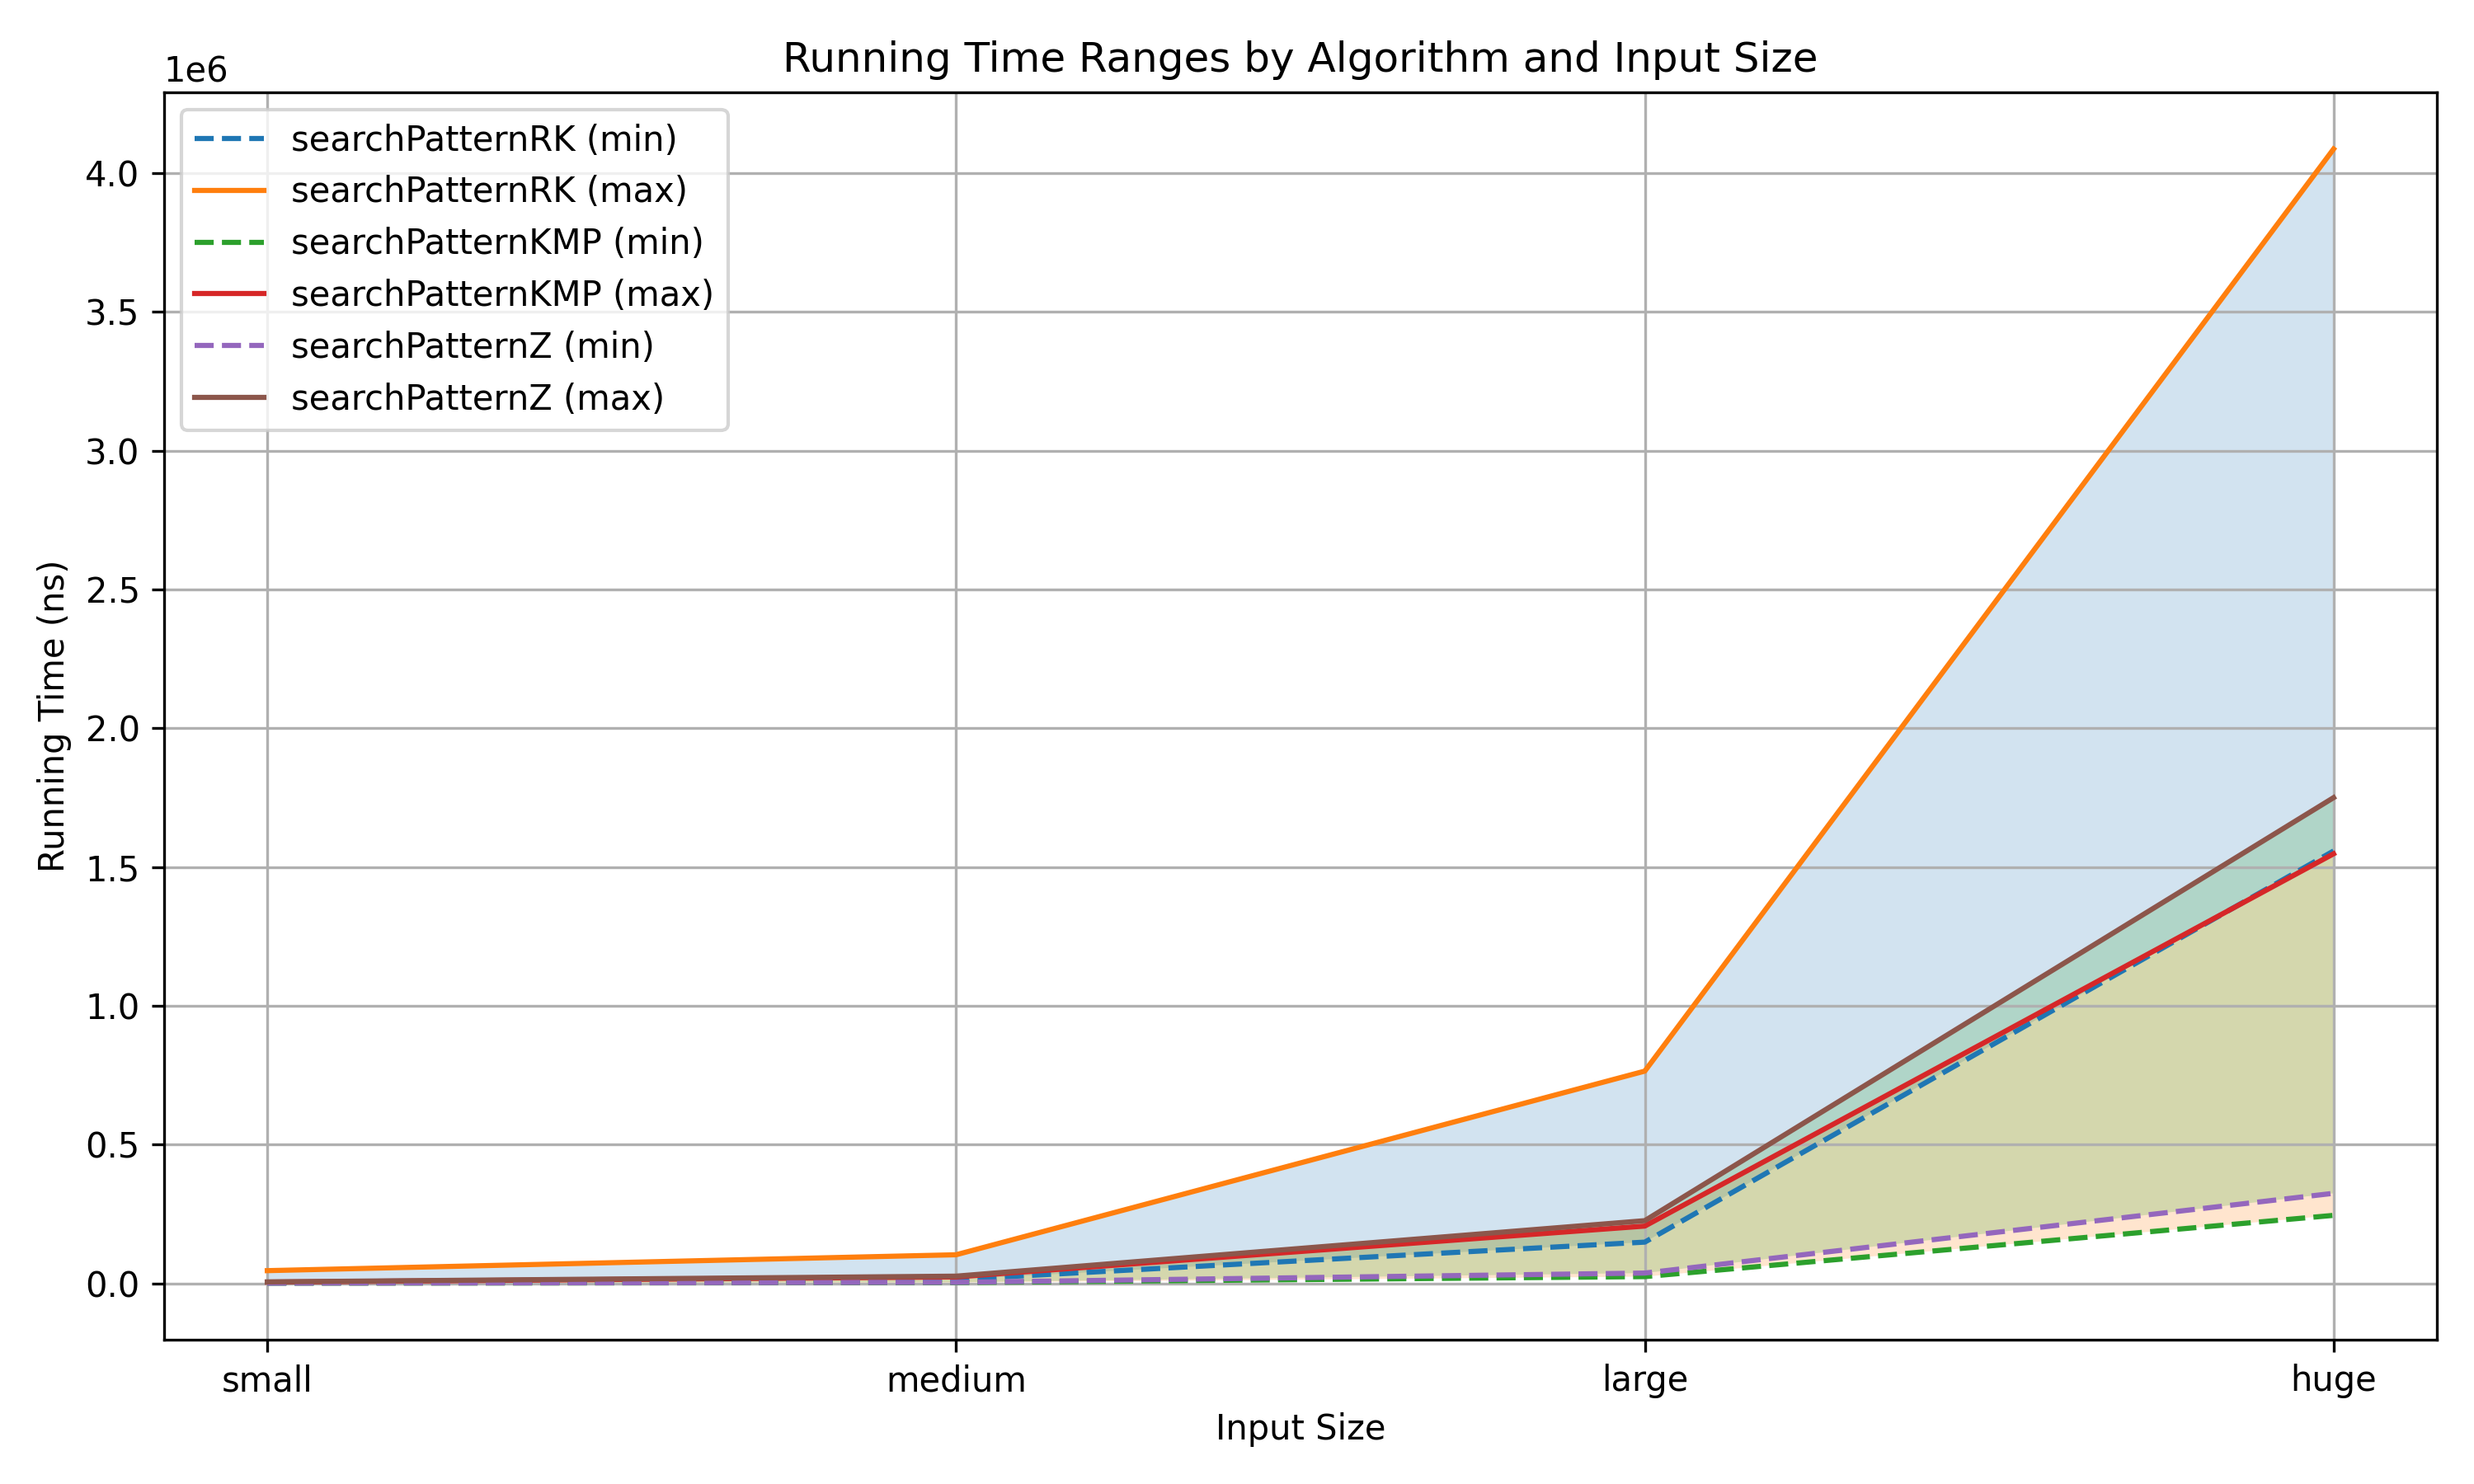
\includegraphics[width=0.7\linewidth]{pattern-stats.png}
  \caption{Pattern‐matching execution times.}
\end{figure}

It is observed that among the given implementations, KMP is the fastest with Z-Function slightly behind and Rabin-Karp being much slower.

\medskip
\textbf{Subpalindrome Detection:}

\begin{table}[H]
  \centering
  \begin{tabular}{@{}lcc@{}}
    \toprule
    Size  & Hash+Binary Search     & Manacher               \\ \midrule
    Small & (13{,}785, 84{,}621)   & (3{,}518, 20{,}550)     \\
    Medium& (174{,}540, 983{,}490) & (30{,}515, 161{,}428)   \\
    Large & (2{,}382{,}988, 5{,}553{,}449) & (389{,}525, 1{,}050{,}119) \\
    Huge  & (28{,}819{,}973, 67{,}110{,}623) & (3{,}411{,}973, 10{,}409{,}500) \\
    \bottomrule
  \end{tabular}
  \caption{Least and highest subpalindrome detection times (nanoseconds).}
\end{table}

\begin{figure}[H]
  \centering
  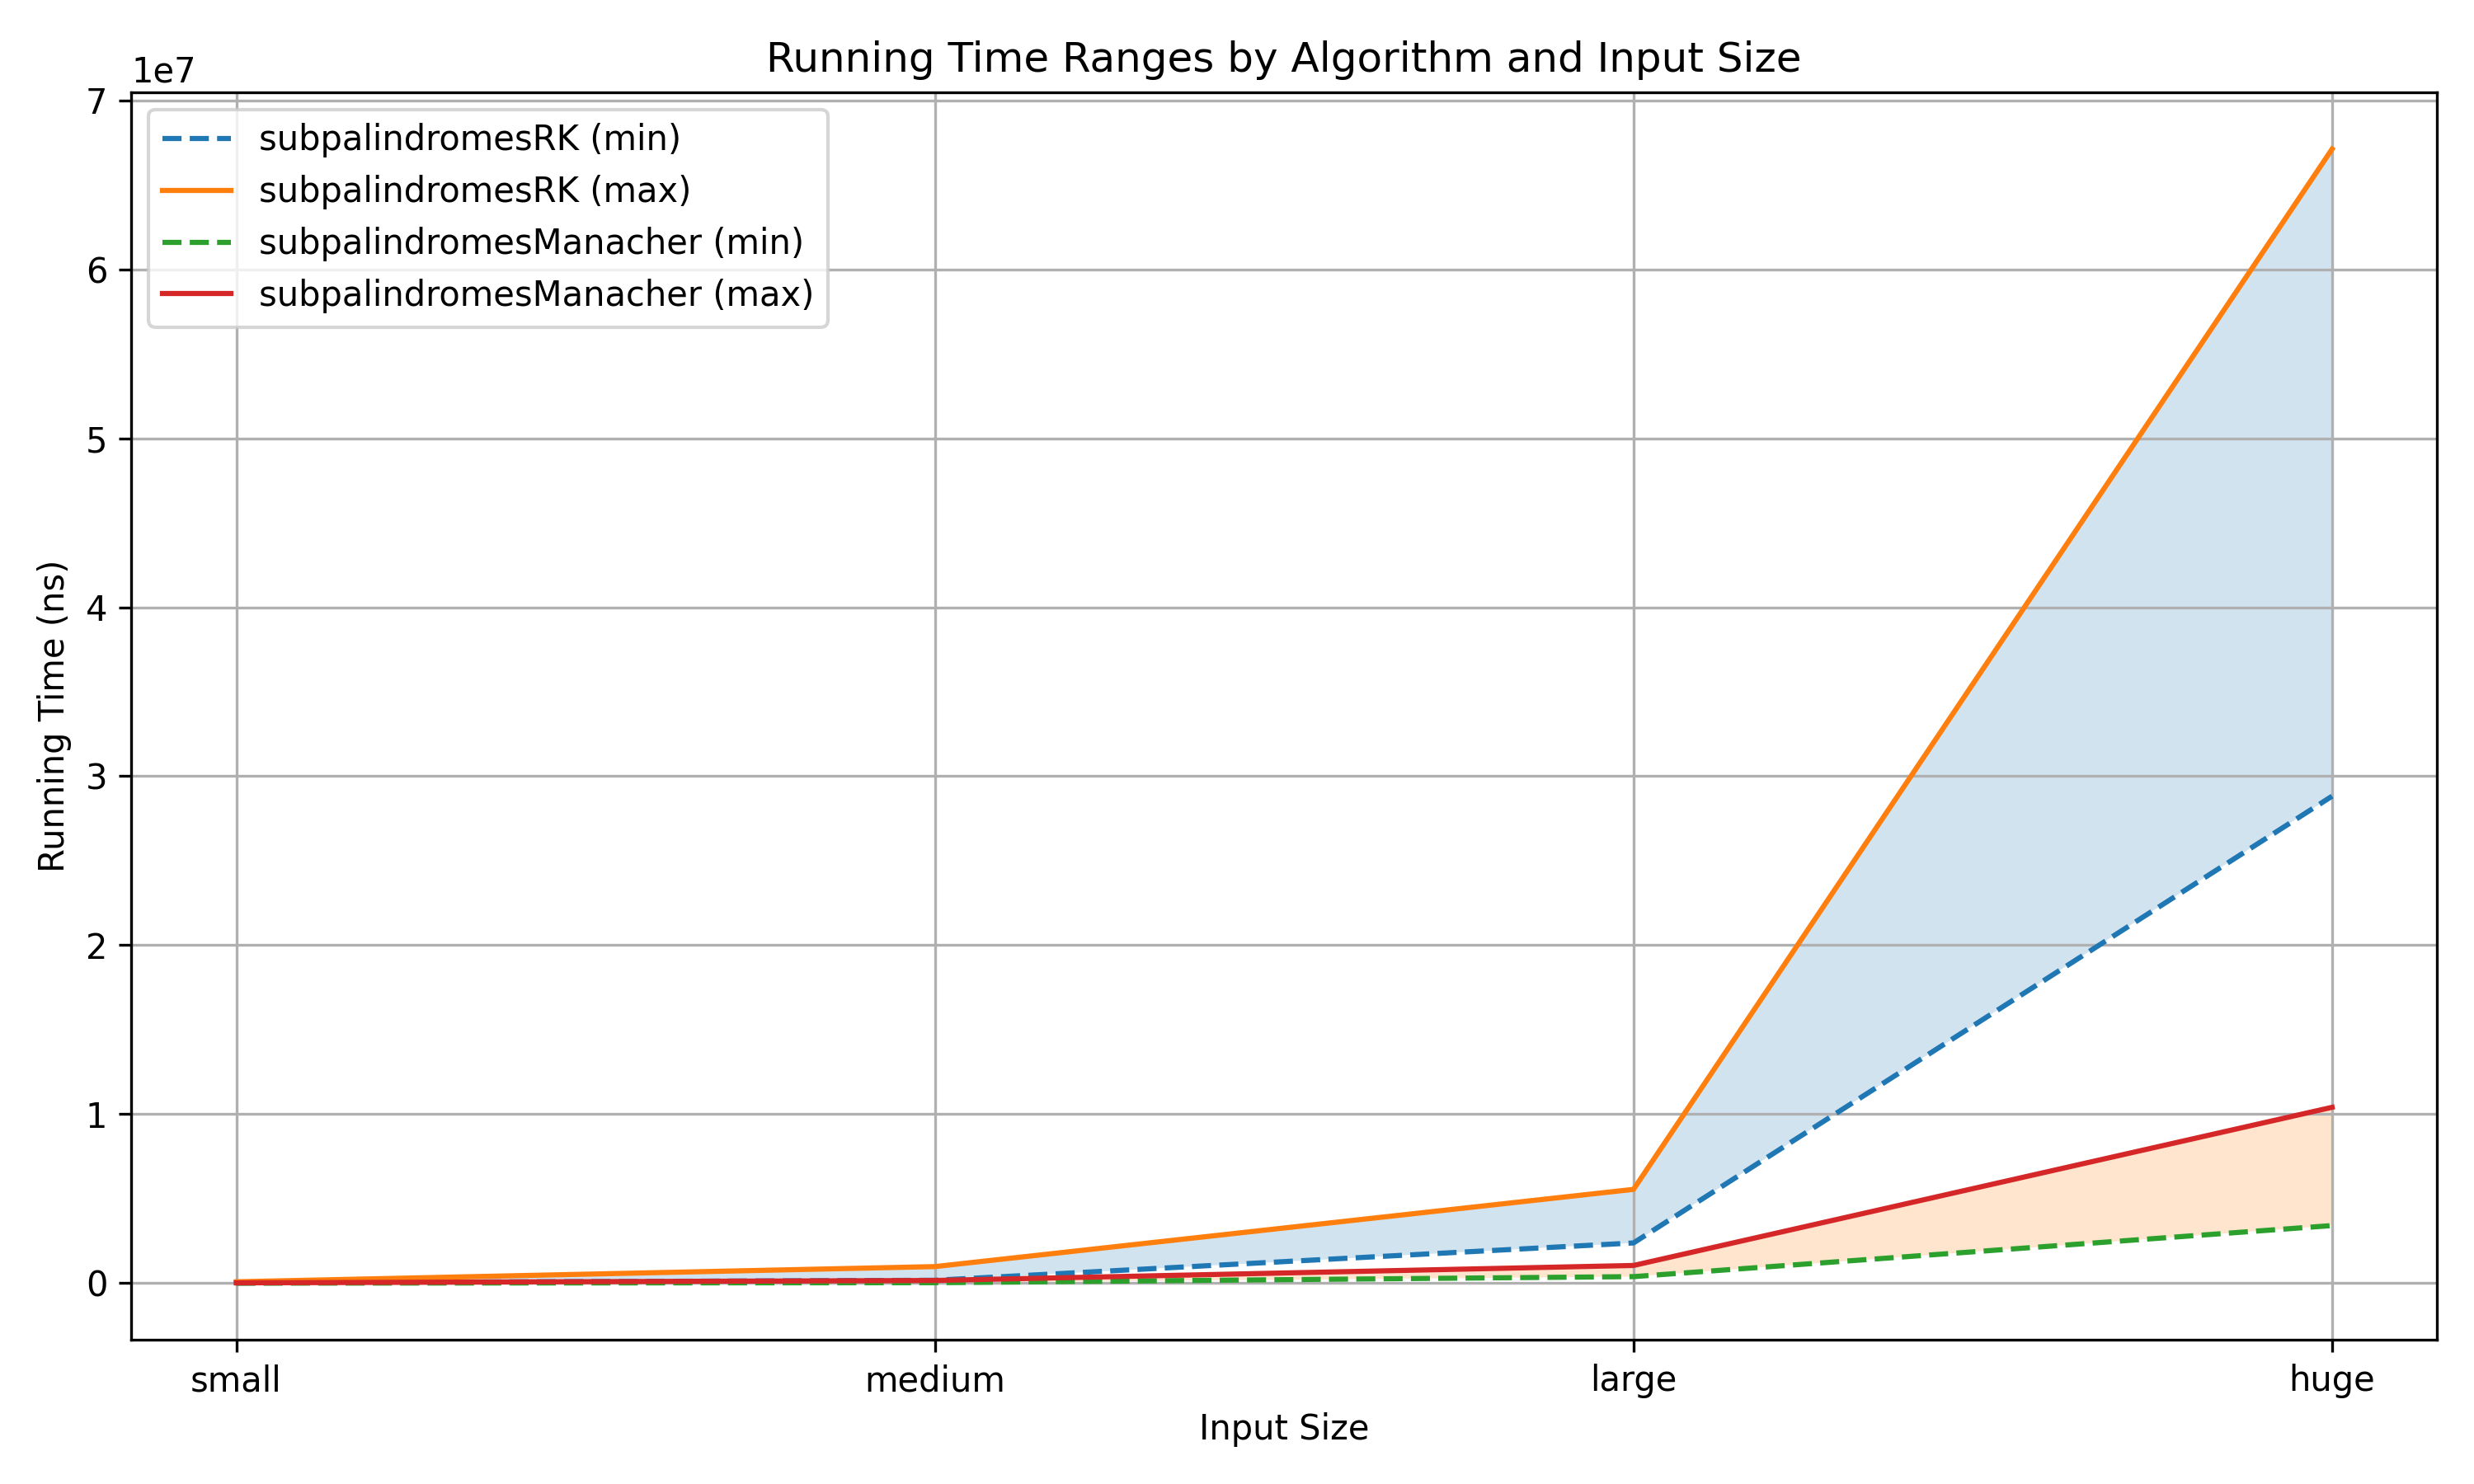
\includegraphics[width=0.7\linewidth]{palindrome-stats.png}
  \caption{Subpalindrome execution times.}
\end{figure}

It is observed that Manacher's algorithm vastly outperforms the $O(n\log n)$ alternative, in line with its linear complexity.

%====================================================
\section{Additional Algorithms}\label{sec:additional-algorithms-detail}

\subsection{Sparse Tables\cite{sparse_table_cp}}
Sparse Table is a data structure, that allows answering static range queries.  
The idea is to store for each range $[i:i + 2^j - 1]$, its result. This can be done efficiently using $O(n\log n)$ memory and time precomputation.  
\begin{itemize}
  \item Precompute: $O(n \log n)$ for an $n$ length array.
  \item Query: $O(\log n)$ or $O(1)$ for \hyperref[https://en.wikipedia.org/wiki/Idempotence]{idempotent functions}
\end{itemize}

\subsection{Square Root Decomposition\cite{sqrt_decomposition_cp}}
Consider the problam of range updates and queries over an array of length $n$.  
Let us break the array into $\left\lceil n/k \right\rceil$ blocks of length $k$ each.\cite{cs166_0}
Maintain a range aggregate for each block.  
Doing so, allows us to performa an update/query in $O(n/k + k)$ time, going over block aggregates and a few extraneous elements to the right/left.   \\
Setting $k = \sqrt n$, we can perform both, queries, and, updates in $\;O(\sqrt n)$ time.

\subsection{Cartesian Tree\cite{cartesian_tree}}
A Cartesian tree is a binary tree that follows the min-heap property. The root is the minimum element and the left/right children are built recursively over the left/right subarrays split.  
It can be constructed in $O(n)$ time using stacks.  

\begin{figure}[H]
  \centering
  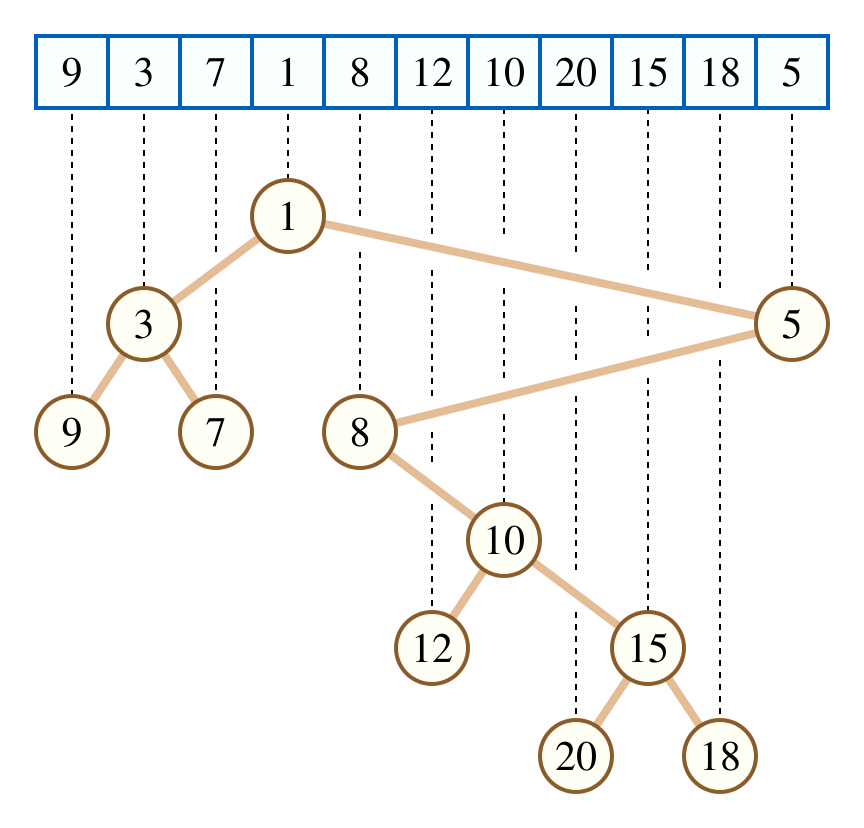
\includegraphics[width=0.4\linewidth]{cartesian_tree.png}
  \caption{A Cartesian tree example.\cite{cartesian_tree}}\label{fig:cartesian}
\end{figure}

\subsection{Method of Four Russians\cite{method_of_four_russians}}
The Method of Four Russians is a technique for speeding up some algorithms over ranges. Particularly, when each cell may take on only a bounded number of possible values.  
\begin{itemize}
  \item Break the problem of size $n$ into subproblems of size $b$, plus some top-level problem of size $n / b$.
  \item This is called a \textbf{macro/micro decomposition}.
  \item Solve all possible subproblems of size $b$.
  \item Solve the overall problem by combining solutions to the micro and macro problems.
  \item Think of it as \textbf{"divide, precompute, and conquer."\cite{cs166_1}}  
\end{itemize}
Typically, $b = O(\log n)$. 

\subsection{Lowest Common Ancestor (LCA)}
The lowest common ancestor problem involves efficiently finding the lowest common ancestor of any two nodes $v_1$ and $v_2$ in a tree, assuming no changes to the tree structure.  
Trivial algorithms can solve this in $O(n^2)$ time by solving for each pair and storing results.  
We shall look at other approaches of solving this efficiently.  

\paragraph{Binary Lifting\cite{lca_binary_lifting}}
Here, for each node, we store it's $2^j$ distance ancestor.  
Given that the $2^0$ ancestor is just the parent and the $2^{j+1}$ distance ancestor is the $2^j$ distance ancestor of the $2^j$ distance ancestor of the node, tranisitions are straightforward.  \\
This allows for $O(N\log N)$ preprocessing for a tree with $N$ nodes.  
Further, each query can be answered in $O(log N)$ time, as follows:
\begin{itemize}
  \item Without loss of generality, let $height(v_1)$ = $u$ $<$ $height(v_2)$ = $v$.
  \item Using at most $\log N$ jumps, we can reach ancestor $v_2'$ from $v_2$, such that $height(v_2')$ = $u$.
  \item We then find the LCA of $v_1$ and $v_2'$, by finding the largest $2^j$ ancestor of each such that they differ, and repeat this until finially the parent of the two nodes found is common.  
  \item This node is the LCA.
\end{itemize}

\paragraph{Farach-Colton \& Bender\cite{lca_farachcoltonbender}}
The algorithm borrows from the Method of Four Russians to break the \hyperref[https://usaco.guide/gold/tree-euler?lang=cpp]{Eulerian tour} of the tree array (of heights) into blocks.  
We divide the array $A$ into blocks of size $K = 0.5\log N$. There are $\left\lceil N/K \right\rceil$ blocks, for each block, store its aggregate, i.e., the minimum, and create a sparse table over these aggregates. The complexity to construct the sparse table is:  
\begin{figure}[H]
  \centering
  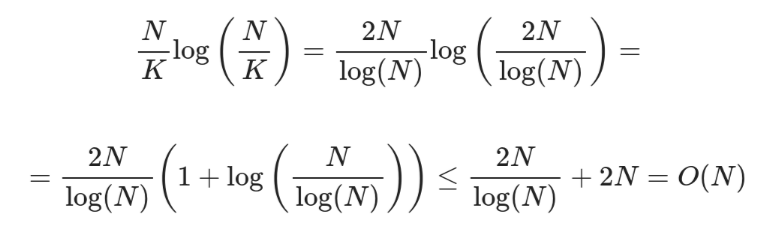
\includegraphics[width=0.7\linewidth]{sparse-calculations.png}
  \caption{Sparse Table Complexity\cite{lca_farachcoltonbender}}
\end{figure}

Minimum over blocks can be solved using the above sparse table.  
For minimum within blocks, we observe that the values in the array being heights computed using the Euler tour of the tree, only differ by $1$, i.e., $+1$ or $-1$, let us represent these by $0$, $1$ respectively.  
Consider subtracting from each element of a block, its first element, this does not change the result of queries (index of minima) inside the block.  
Because the blocks are so small, there are only a handful of possible sequences:  

\begin{figure}[H]
  \centering
  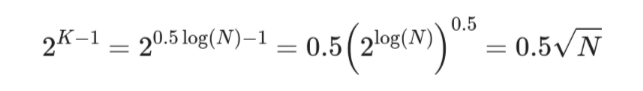
\includegraphics[width=0.7\linewidth]{block-calculations.png}
  \caption{Block Possibilities Count\cite{lca_farachcoltonbender}}
\end{figure}

Thus, the number of different blocks is at most $O(\sqrt N)$, and therefore results of range minimum queries over them can be precomputed in time: $$\;O(\sqrt N \cdot K^2) = \;O(\sqrt N\cdot \log^2 N)) = O(N)$$
Mapping between blocks and results can be stored in an array $block[bitmask][left][right]$, storing the results of the block over its subarray $[left,right]$.

\paragraph{Note}
An interesting implication of the above is a different method for the static range-minium-query (RMQ) problem.\cite{lca_rmq}  
By constructing a cartesian tree on the input array (of length $n$), we can solve the RMQ problem with $O(n)$ precomputation and $O(1)$ time per query.  
Query resolution is equivalent here to finding the LCA over a range.

%====================================================
\section{Docs}\label{sec:docs}

\subsection{Analysis}
Algorithms' algorithmic complexity analysis and correctness guarantees where relevant are included.  

\subsection{Benchmarking}
Real world performance of algorithms/programs depends on a variety of factors such as inputs, infrastructure capabilities, environment, program optimizations, etc.  
Theoretically optimal algorithms aren't necessarily the best solutions in practice. To understand and study these differences, we benchmark programs as follows: \\ 
Program running times may vary, and are considered to be random variables.
\begin{itemize}
    \item We would like to find statistical guarantees about the expected running times.
    \item Since expectation and variance are unknown, concentration inequalities cannot be used to estimate tight bounds on expectation.
    \item Considering the above, we instead study the $n$-th percentile performance with strict statistical guarantees, particularly the median.
\end{itemize}

\paragraph{Benchmarking Pipeline}
Assuming program running times are random variables sampled from a distribution, the following ensues.
\begin{itemize}
    \item Run the program $T$ times and note the running times, $t_1, \dots, t_n$.
    \item Find the least and highest running times:
    \begin{align*}
        lrt &= \min_{1 \leq i \leq n} (t_i) \\
        hrt &= \max_{1 \leq i \leq n} (t_i)
    \end{align*}
    \item \textit{Claim:} The median running time lies in the range $[lrt, hrt]$ with probability $1 - 2^{-(T - 1)}$.
    \item \textit{Proof:}
    \begin{align*}
        \text{Pr}[\text{median} \in [lrt, hrt]] &= 1 - \text{Pr}[\text{median} < lrt \mid hrt < \text{median}] \\
                                                &= 1 - \text{Pr}[\text{median} < lrt] - \text{Pr}[hrt < \text{median}] \quad \text{(since the events are disjoint)} \\
                                                &= 1 - 2^{-T} - 2^{-T} \quad \text{(since probability that a single execution is on either side } = 2^{-1}) \\
                                                &= 1 - 2^{-(T - 1)}
    \end{align*}
    \item Similar arguments can be used to find $n^{th}$ percentile statistics.
\end{itemize}

\paragraph{Comparing Algorithms}
While exact comparisons between algorithms on the basis of the overlapping bounds are not feasible, a direct comparison can instead be made as follows:
\begin{itemize}
    \item For each pair of algorithms, run both on the same set of inputs and compare running times.
    \item If either comes ahead by at least a margin (say, $5\%$), we can attribute that to the algorithm's efficiency.
    \item If not, the result for the same can be marked inconclusive.
\end{itemize}
While the above is more direct, we have used the bounds as indicative of performance and instead performed comparison across all algorithms rather than pairwise analysis.

\subsection{Optimizations}
All C++ benchmarks compiled with \texttt{-Ofast -march=native} flags.

\subsection{System Information}
\begin{itemize}
  \item Processor: Intel(R) Core(TM) Ultra 9 185H
  \item Operating System: Linux 6.14.5
  \item Language Versions: C++23 (gcc 15.1.1), Python 3.13.3, Bash 5.2.37
\end{itemize}

\section{Conclusion}
Through this study, we benchmarked and analyzed the nuances between algorithms, where theoretical complexity didn't always imply algorithmic superiority. \\
The input size and values also contributed in turn to performance. We studied the running times under a statistical lens with mathematical guarantees on bounds. \\
\subsection{Results}
\begin{itemize}
  \item Random-hash or xor-hash were poor in comparison to polynomial hashing and fnv-1a hash.
  \item Fenwick trees outperformed both iterative and recursive versions of Segment trees, where the iterative version was only slightly behind.
  \item The insertion+quicksort hybrid performed best across all input sizes with insertion sort performing equally well on small inputs and quicksort only lagging behind slightly on larger inputs and merge sort lagging by a margin.
  \item KMP and Z-Function performed similarly on pattern matching with Rabin-Karp lagging behind, while Manacher's algorithm outperformed Rabin-Karp+Binary-Search by a margin.
\end{itemize}

\subsection{Future Scope}
The practical study of algorithms can be further extended to other algorithms, and particularly those with hardware specific optimizations.\\
Sorting\cite{google_vectorized_quicksort} and Pattern matching\cite{stackoverflow_stringfind_complexity}, problems we have considered are already known to benefit from the same. \\
In addition, work from \hyperref[http://sereja.me/]{Sergey Slotin} on data structures\cite{sslotin_book} such as segment trees \cite{wide_segment_tree} is another area of study for practical performance. \\
Deep understanding of systems programming languages, assembly and hardware optimizations are expected to dive into these directions.  \\
Another direction for work is to consider scaling of performance upon parallelization, how well do algorithms perform with horizontal scaling of resources?

\begin{thebibliography}{50}

  \bibitem{gcc_optimization_pragmas}
  ``GCC Optimization Pragmas,''
  \url{https://nor-blog.pages.dev/posts/2021-10-26-gcc-optimization-pragmas/},
  [Online; accessed 15-May-2025].
  
  \bibitem{avalanche_effect}
  ``Avalanche effect,''
  \emph{Wikipedia},
  \url{https://en.wikipedia.org/wiki/Avalanche_effect},
  [Online; accessed 15-May-2025].
  
  \bibitem{string_hashing_cp}
  ``String Hashing,''
  \emph{CP-Algorithms},
  \url{https://cp-algorithms.com/string/string-hashing.html},
  [Online; accessed 15-May-2025].

  \bibitem{fnv_hash}
  ``FNV hash function,''
  \emph{Wikipedia},
  \url{https://en.wikipedia.org/wiki/Fowler%E2%80%93Noll%E2%80%93Vo_hash_function},
  [Online; accessed 15-May-2025].
  
  \bibitem{universal_hashing}
  ``Universal hashing,''
  \emph{Wikipedia},
  \url{https://en.wikipedia.org/wiki/Universal_hashing},
  [Online; accessed 15-May-2025].
  
  \bibitem{fenwick_tree_cp}
  ``Fenwick Tree,''
  \emph{CP-Algorithms},
  \url{https://cp-algorithms.com/data_structures/fenwick.html},
  [Online; accessed 15-May-2025].
  
  \bibitem{segment_tree_cp}
  ``Segment Tree,''
  \emph{CP-Algorithms},
  \url{https://cp-algorithms.com/data_structures/segment_tree.html},
  [Online; accessed 15-May-2025].
  
  \bibitem{iterative_segment_tree}
  ``Iterative Segment Tree,''
  \emph{Codeforces Blog},
  \url{https://codeforces.com/blog/entry/18051},
  [Online; accessed 15-May-2025].
  
  \bibitem{fenwick_tree_rmq}
  ``Fenwick Tree - Range Minimum Queries,''
  \emph{IO Informatics}, vol.~9, pp.~39--44, 2015,
  \url{https://ioinformatics.org/journal/v9_2015_39_44.pdf},
  [Online; accessed 15-May-2025].
  
  \bibitem{insertion_sort_wiki}
  ``Insertion sort,''
  \emph{Wikipedia},
  \url{https://en.wikipedia.org/wiki/Insertion_sort},
  [Online; accessed 15-May-2025].
  
  \bibitem{merge_sort_wiki}
  ``Merge sort,''
  \emph{Wikipedia},
  \url{https://en.wikipedia.org/wiki/Merge_sort},
  [Online; accessed 15-May-2025].
  
  \bibitem{quicksort_wiki}
  ``Quicksort,''
  \emph{Wikipedia},
  \url{https://en.wikipedia.org/wiki/Quicksort},
  [Online; accessed 15-May-2025].
  
  \bibitem{dual_pivot_quicksort_jdk}
  ``DualPivotQuicksort.java,''
  \emph{OpenJDK},
  \url{https://github.com/openjdk/jdk/blob/master/src/java.base/share/classes/java/util/DualPivotQuicksort.java},
  [Online; accessed 15-May-2025].
  
  \bibitem{dual_pivot_quicksort_so}
  ``What's the difference of dual pivot quick sort and quick sort?''
  \emph{Stack Overflow},
  \url{https://stackoverflow.com/questions/20917617/whats-the-difference-of-dual-pivot-quick-sort-and-quick-sort},
  [Online; accessed 15-May-2025].
  
  \bibitem{kmp_cp}
  ``KMP (Knuth-Morris-Pratt),''
  \emph{CP-Algorithms},
  \url{https://cp-algorithms.com/string/prefix-function.html},
  [Online; accessed 15-May-2025].
  
  \bibitem{manacher_cp}
  ``Manacher's Algorithm - Finding all sub-palindromes in $O(N)$,''
  \emph{CP-Algorithms},
  \url{https://cp-algorithms.com/string/manacher.html},
  [Online; accessed 15-May-2025].
  
  \bibitem{rabin_karp_cp}
  ``Rabin-Karp,''
  \emph{CP-Algorithms},
  \url{https://cp-algorithms.com/string/rabin-karp.html},
  [Online; accessed 15-May-2025].
  
  \bibitem{z_function_cp}
  ``Z-function,''
  \emph{CP-Algorithms},
  \url{https://cp-algorithms.com/string/z-function.html},
  [Online; accessed 15-May-2025].
  
  \bibitem{sparse_table_cp}
  ``Sparse Table,''
  \emph{CP-Algorithms},
  \url{https://cp-algorithms.com/data_structures/sparse-table.html},
  [Online; accessed 15-May-2025].
  
  \bibitem{cs166_0}
  ``CS166: Data Structures (Lecture 0),''
  \emph{Wayback Machine}, Aug. 12, 2023,
  \url{https://web.archive.org/web/20230812194808/http://web.stanford.edu/class/cs166/lectures/00/Small00.pdf},
  [Online; accessed 15-May-2025].
  
  \bibitem{cs166_1}
  ``CS166: Data Structures (Lecture 1),''
  \emph{Wayback Machine}, Apr. 22, 2024,
  \url{https://web.archive.org/web/20240422013245/https://web.stanford.edu/class/cs166/lectures/01/Small01.pdf},
  [Online; accessed 15-May-2025].

  \bibitem{cartesian_tree}
  ``Cartesian Tree,''
  \emph{Wikipedia}
  \url{https://en.wikipedia.org/wiki/Cartesian_tree},
  [Online; accessed 15-May-2025]
  
  \bibitem{method_of_four_russians}
  ``Method of Four Russians,''
  \emph{Wikipedia},
  \url{https://en.wikipedia.org/wiki/Method_of_Four_Russians},
  [Online; accessed 15-May-2025].
  
  \bibitem{sqrt_decomposition_cp}
  ``Sqrt Decomposition,''
  \emph{CP-Algorithms},
  \url{https://cp-algorithms.com/data_structures/sqrt_decomposition.html},
  [Online; accessed 15-May-2025].
  
  \bibitem{lca_binary_lifting}
  ``LCA - Binary Lifting,''
  \emph{CP-Algorithms},
  \url{https://cp-algorithms.com/graph/lca_binary_lifting.html},
  [Online; accessed 15-May-2025].
  
  \bibitem{lca_farachcoltonbender}
  ``LCA - Farach-Colton and Bender,''
  \emph{CP-Algorithms},
  \url{https://cp-algorithms.com/graph/lca_farachcoltonbender.html},
  [Online; accessed 15-May-2025].
  
  \bibitem{lca_rmq}
  ``LCA - Reduction to RMQ. Linear Algorithm,''
  \emph{CP-Algorithms},
  \url{https://cp-algorithms.com/graph/rmq_linear.html},
  [Online; accessed 15-May-2025].

  \bibitem{google_vectorized_quicksort}
  ``Vectorized and performance portable Quicksort,''
  \emph{Google Open Source Blog}, June 2022,
  \url{https://opensource.googleblog.com/2022/06/Vectorized%20and%20performance%20portable%20Quicksort.html},
  [Online; accessed 15-May-2025].

  \bibitem{stackoverflow_stringfind_complexity}
  ``C++ string::find() complexity,''
  \emph{Stack Overflow}, Apr. 26, 2012,
  \url{https://stackoverflow.com/questions/8869605/c-stringfind-complexity},
  [Online; accessed 15-May-2025].

  
  \bibitem{sslotin_book}
  ``SIMD Algorithms,''
  \emph{Codeforces},
  \url{https://codeforces.com/blog/entry/99790},
  [Online; accessed 15-May-2025].

  \bibitem{wide_segment_tree}
  ``Even more efficient but not so easy Segment Trees,''
  \emph{Codeforces},
  \url{https://codeforces.com/blog/entry/100454},
  [Online; accessed 15-May-2025].
\end{thebibliography}

\end{document}